% Options for packages loaded elsewhere
\PassOptionsToPackage{unicode}{hyperref}
\PassOptionsToPackage{hyphens}{url}
%
\documentclass[
]{article}
\usepackage{amsmath,amssymb}
\usepackage{lmodern}
\usepackage{ifxetex,ifluatex}
\ifnum 0\ifxetex 1\fi\ifluatex 1\fi=0 % if pdftex
  \usepackage[T1]{fontenc}
  \usepackage[utf8]{inputenc}
  \usepackage{textcomp} % provide euro and other symbols
\else % if luatex or xetex
  \usepackage{unicode-math}
  \defaultfontfeatures{Scale=MatchLowercase}
  \defaultfontfeatures[\rmfamily]{Ligatures=TeX,Scale=1}
\fi
% Use upquote if available, for straight quotes in verbatim environments
\IfFileExists{upquote.sty}{\usepackage{upquote}}{}
\IfFileExists{microtype.sty}{% use microtype if available
  \usepackage[]{microtype}
  \UseMicrotypeSet[protrusion]{basicmath} % disable protrusion for tt fonts
}{}
\makeatletter
\@ifundefined{KOMAClassName}{% if non-KOMA class
  \IfFileExists{parskip.sty}{%
    \usepackage{parskip}
  }{% else
    \setlength{\parindent}{0pt}
    \setlength{\parskip}{6pt plus 2pt minus 1pt}}
}{% if KOMA class
  \KOMAoptions{parskip=half}}
\makeatother
\usepackage{xcolor}
\IfFileExists{xurl.sty}{\usepackage{xurl}}{} % add URL line breaks if available
\IfFileExists{bookmark.sty}{\usepackage{bookmark}}{\usepackage{hyperref}}
\hypersetup{
  pdftitle={Association between weight history and PRL params},
  pdfauthor={Corrado Caudek},
  hidelinks,
  pdfcreator={LaTeX via pandoc}}
\urlstyle{same} % disable monospaced font for URLs
\usepackage[margin=1in]{geometry}
\usepackage{color}
\usepackage{fancyvrb}
\newcommand{\VerbBar}{|}
\newcommand{\VERB}{\Verb[commandchars=\\\{\}]}
\DefineVerbatimEnvironment{Highlighting}{Verbatim}{commandchars=\\\{\}}
% Add ',fontsize=\small' for more characters per line
\usepackage{framed}
\definecolor{shadecolor}{RGB}{248,248,248}
\newenvironment{Shaded}{\begin{snugshade}}{\end{snugshade}}
\newcommand{\AlertTok}[1]{\textcolor[rgb]{0.94,0.16,0.16}{#1}}
\newcommand{\AnnotationTok}[1]{\textcolor[rgb]{0.56,0.35,0.01}{\textbf{\textit{#1}}}}
\newcommand{\AttributeTok}[1]{\textcolor[rgb]{0.77,0.63,0.00}{#1}}
\newcommand{\BaseNTok}[1]{\textcolor[rgb]{0.00,0.00,0.81}{#1}}
\newcommand{\BuiltInTok}[1]{#1}
\newcommand{\CharTok}[1]{\textcolor[rgb]{0.31,0.60,0.02}{#1}}
\newcommand{\CommentTok}[1]{\textcolor[rgb]{0.56,0.35,0.01}{\textit{#1}}}
\newcommand{\CommentVarTok}[1]{\textcolor[rgb]{0.56,0.35,0.01}{\textbf{\textit{#1}}}}
\newcommand{\ConstantTok}[1]{\textcolor[rgb]{0.00,0.00,0.00}{#1}}
\newcommand{\ControlFlowTok}[1]{\textcolor[rgb]{0.13,0.29,0.53}{\textbf{#1}}}
\newcommand{\DataTypeTok}[1]{\textcolor[rgb]{0.13,0.29,0.53}{#1}}
\newcommand{\DecValTok}[1]{\textcolor[rgb]{0.00,0.00,0.81}{#1}}
\newcommand{\DocumentationTok}[1]{\textcolor[rgb]{0.56,0.35,0.01}{\textbf{\textit{#1}}}}
\newcommand{\ErrorTok}[1]{\textcolor[rgb]{0.64,0.00,0.00}{\textbf{#1}}}
\newcommand{\ExtensionTok}[1]{#1}
\newcommand{\FloatTok}[1]{\textcolor[rgb]{0.00,0.00,0.81}{#1}}
\newcommand{\FunctionTok}[1]{\textcolor[rgb]{0.00,0.00,0.00}{#1}}
\newcommand{\ImportTok}[1]{#1}
\newcommand{\InformationTok}[1]{\textcolor[rgb]{0.56,0.35,0.01}{\textbf{\textit{#1}}}}
\newcommand{\KeywordTok}[1]{\textcolor[rgb]{0.13,0.29,0.53}{\textbf{#1}}}
\newcommand{\NormalTok}[1]{#1}
\newcommand{\OperatorTok}[1]{\textcolor[rgb]{0.81,0.36,0.00}{\textbf{#1}}}
\newcommand{\OtherTok}[1]{\textcolor[rgb]{0.56,0.35,0.01}{#1}}
\newcommand{\PreprocessorTok}[1]{\textcolor[rgb]{0.56,0.35,0.01}{\textit{#1}}}
\newcommand{\RegionMarkerTok}[1]{#1}
\newcommand{\SpecialCharTok}[1]{\textcolor[rgb]{0.00,0.00,0.00}{#1}}
\newcommand{\SpecialStringTok}[1]{\textcolor[rgb]{0.31,0.60,0.02}{#1}}
\newcommand{\StringTok}[1]{\textcolor[rgb]{0.31,0.60,0.02}{#1}}
\newcommand{\VariableTok}[1]{\textcolor[rgb]{0.00,0.00,0.00}{#1}}
\newcommand{\VerbatimStringTok}[1]{\textcolor[rgb]{0.31,0.60,0.02}{#1}}
\newcommand{\WarningTok}[1]{\textcolor[rgb]{0.56,0.35,0.01}{\textbf{\textit{#1}}}}
\usepackage{graphicx}
\makeatletter
\def\maxwidth{\ifdim\Gin@nat@width>\linewidth\linewidth\else\Gin@nat@width\fi}
\def\maxheight{\ifdim\Gin@nat@height>\textheight\textheight\else\Gin@nat@height\fi}
\makeatother
% Scale images if necessary, so that they will not overflow the page
% margins by default, and it is still possible to overwrite the defaults
% using explicit options in \includegraphics[width, height, ...]{}
\setkeys{Gin}{width=\maxwidth,height=\maxheight,keepaspectratio}
% Set default figure placement to htbp
\makeatletter
\def\fps@figure{htbp}
\makeatother
\setlength{\emergencystretch}{3em} % prevent overfull lines
\providecommand{\tightlist}{%
  \setlength{\itemsep}{0pt}\setlength{\parskip}{0pt}}
\setcounter{secnumdepth}{-\maxdimen} % remove section numbering
\ifluatex
  \usepackage{selnolig}  % disable illegal ligatures
\fi

\title{Association between weight history and PRL params}
\author{\href{https://ccaudek.github.io/}{Corrado Caudek}}
\date{First version 08:21:00 2021. Last modified 2021-06-16}

\begin{document}
\maketitle

Purpose: to determine whether the PRL hDDMrl parameters can be
associated to the behavioral characteristics of participants, after
accounting for the individual differences explained by the
questionnaires data.

\begin{verbatim}
## here() starts at /Users/corrado/Documents/papers/ED_patients
\end{verbatim}

\begin{verbatim}
## CmdStan path set to: /Users/corrado/cmdstan
\end{verbatim}

\begin{verbatim}
## Warning in find_bad_controls(THRESHOLD): NA introdotti per coercizione
\end{verbatim}

\begin{verbatim}
## `summarise()` has grouped output by 'is_patient'. You can override using the `.groups` argument.
\end{verbatim}

\begin{verbatim}
## [1] 176
\end{verbatim}

\begin{verbatim}
## [1] 38
\end{verbatim}

\begin{verbatim}
##     subj_idx      subj_code           a_neither          v_food      
##  Min.   :  0.0   Length:131         Min.   :0.7961   Min.   :-5.315  
##  1st Qu.: 72.5   Class :character   1st Qu.:1.1191   1st Qu.: 1.257  
##  Median :141.0   Mode  :character   Median :1.3104   Median : 1.928  
##  Mean   :147.7                      Mean   :1.3008   Mean   : 2.007  
##  3rd Qu.:221.0                      3rd Qu.:1.4680   3rd Qu.: 2.695  
##  Max.   :302.0                      Max.   :1.7508   Max.   : 5.786  
##                                                      NA's   :7       
##     v_social          t_food           t_social          z_food      
##  Min.   :0.8035   Min.   :0.06597   Min.   :0.0757   Min.   :0.4666  
##  1st Qu.:1.7820   1st Qu.:0.14400   1st Qu.:0.1546   1st Qu.:0.4887  
##  Median :2.2819   Median :0.18360   Median :0.1965   Median :0.4944  
##  Mean   :2.4186   Mean   :0.18983   Mean   :0.1973   Mean   :0.4943  
##  3rd Qu.:3.1090   3rd Qu.:0.22966   3rd Qu.:0.2281   3rd Qu.:0.5007  
##  Max.   :7.5216   Max.   :0.60062   Max.   :0.5384   Max.   :0.5172  
##  NA's   :10       NA's   :7         NA's   :10       NA's   :7       
##     z_social      alpha_neg_food   alpha_neg_social alpha_pos_food   
##  Min.   :0.4702   Min.   :-6.167   Min.   :-2.766   Min.   :-7.2959  
##  1st Qu.:0.4918   1st Qu.: 1.254   1st Qu.: 1.615   1st Qu.:-0.7276  
##  Median :0.4974   Median : 4.222   Median : 4.688   Median : 1.2491  
##  Mean   :0.4970   Mean   : 3.442   Mean   : 3.686   Mean   : 0.8231  
##  3rd Qu.:0.5030   3rd Qu.: 5.833   3rd Qu.: 5.878   3rd Qu.: 2.5662  
##  Max.   :0.5220   Max.   : 6.877   Max.   : 7.106   Max.   : 4.1822  
##  NA's   :10       NA's   :7        NA's   :10       NA's   :7        
##  alpha_pos_social    bsq14_tot        ros_tot      dass21_stress   
##  Min.   :-3.1442   Min.   :14.00   Min.   :11.00   Min.   : 0.000  
##  1st Qu.: 0.0122   1st Qu.:29.00   1st Qu.:17.00   1st Qu.: 7.000  
##  Median : 2.1575   Median :46.00   Median :23.00   Median : 9.000  
##  Mean   : 1.7165   Mean   :45.23   Mean   :22.68   Mean   : 9.867  
##  3rd Qu.: 3.2640   3rd Qu.:58.00   3rd Qu.:27.00   3rd Qu.:13.000  
##  Max.   : 4.3755   Max.   :79.00   Max.   :39.00   Max.   :19.000  
##  NA's   :10        NA's   :18      NA's   :18      NA's   :18      
##  dass21_anxiety     dass21_dep          sias           mps_ps     
##  Min.   : 0.000   Min.   : 0.000   Min.   : 5.00   Min.   :11.00  
##  1st Qu.: 3.000   1st Qu.: 4.000   1st Qu.:19.00   1st Qu.:19.00  
##  Median : 5.000   Median : 7.000   Median :31.00   Median :22.00  
##  Mean   : 5.699   Mean   : 8.018   Mean   :30.62   Mean   :22.42  
##  3rd Qu.: 8.000   3rd Qu.:12.000   3rd Qu.:41.00   3rd Qu.:26.00  
##  Max.   :16.000   Max.   :19.000   Max.   :64.00   Max.   :34.00  
##  NA's   :18       NA's   :18       NA's   :18      NA's   :18     
##      mps_o          mps_cmd         mps_pepc        orto_tot    
##  Min.   :10.00   Min.   :19.00   Min.   : 8.00   Min.   : 7.00  
##  1st Qu.:20.00   1st Qu.:36.00   1st Qu.:14.00   1st Qu.:15.00  
##  Median :22.00   Median :43.00   Median :18.00   Median :19.00  
##  Mean   :22.24   Mean   :43.99   Mean   :18.49   Mean   :18.14  
##  3rd Qu.:26.00   3rd Qu.:51.00   3rd Qu.:22.00   3rd Qu.:22.00  
##  Max.   :30.00   Max.   :67.00   Max.   :37.00   Max.   :26.00  
##  NA's   :18      NA's   :18      NA's   :18      NA's   :18     
##     dieting          bulimia        oral_control    eat26_at_risk   
##  Min.   : 0.000   Min.   : 3.000   Min.   : 0.000   Min.   :0.0000  
##  1st Qu.: 2.000   1st Qu.: 3.000   1st Qu.: 0.000   1st Qu.:0.0000  
##  Median : 4.000   Median : 3.000   Median : 1.000   Median :0.0000  
##  Mean   : 8.324   Mean   : 5.481   Mean   : 3.093   Mean   :0.2685  
##  3rd Qu.:11.000   3rd Qu.: 8.000   3rd Qu.: 3.000   3rd Qu.:1.0000  
##  Max.   :33.000   Max.   :13.000   Max.   :19.000   Max.   :1.0000  
##  NA's   :23       NA's   :23       NA's   :23       NA's   :23      
##    is_patient        group               eat26     
##  Min.   :0.0000   Length:131         Min.   : 3.0  
##  1st Qu.:0.0000   Class :character   1st Qu.: 6.0  
##  Median :0.0000   Mode  :character   Median :10.0  
##  Mean   :0.2901                      Mean   :16.9  
##  3rd Qu.:1.0000                      3rd Qu.:23.0  
##  Max.   :1.0000                      Max.   :59.0  
##                                      NA's   :23
\end{verbatim}

\begin{verbatim}
## 
##  0  1  2 
## 70 12 38
\end{verbatim}

\begin{verbatim}
## 
##  0  1  2 
## 70 12 38
\end{verbatim}

\begin{verbatim}
## [1] "ordered" "factor"
\end{verbatim}

\begin{verbatim}
## 
##  0  1  2 
## 56 10 37
\end{verbatim}

\begin{verbatim}
## 
##  0  2 
## 56 37
\end{verbatim}

\begin{verbatim}
## Warning in if (class(df[, colName]) == "integer" | class(df[, colName]) == : la
## condizione ha lunghezza > 1 e solo il primo elemento sarà utilizzato
\end{verbatim}

\begin{verbatim}
## 
##  0  1 
## 56 37
\end{verbatim}

\begin{verbatim}
## Warning in if (class(df[, colName]) == "integer" | class(df[, colName]) == : la
## condizione ha lunghezza > 1 e solo il primo elemento sarà utilizzato
\end{verbatim}

\begin{verbatim}
## 
##  0  1 
## 75 37
\end{verbatim}

\begin{verbatim}
## Warning: Removed 21 rows containing non-finite values (stat_density).
\end{verbatim}

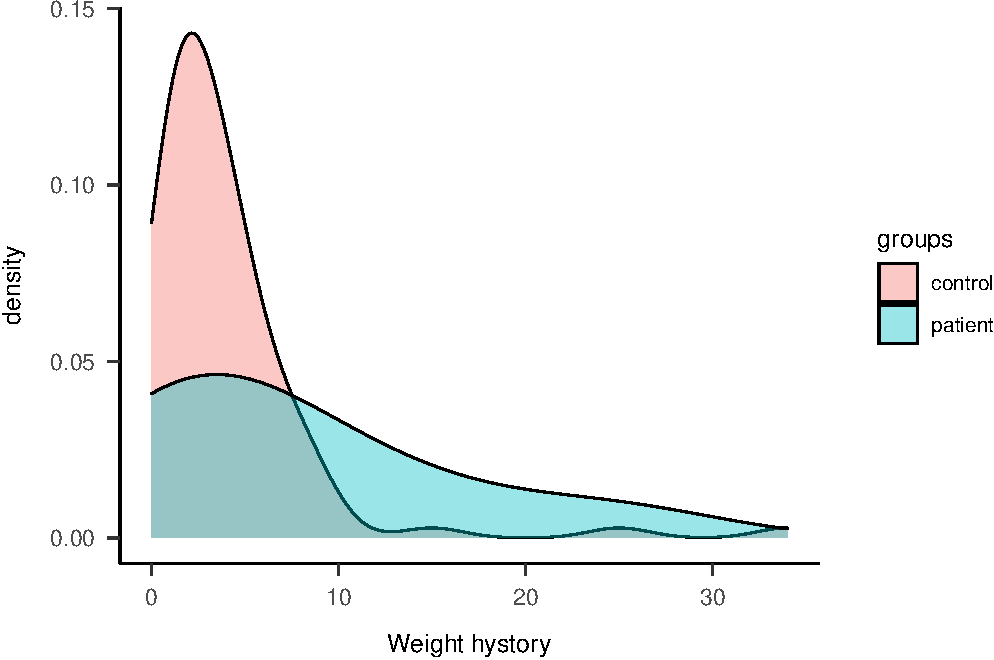
\includegraphics{046_weight_history_alpha_files/figure-latex/unnamed-chunk-3-1.pdf}

\begin{verbatim}
## Warning: Removed 20 rows containing non-finite values (stat_density).
\end{verbatim}

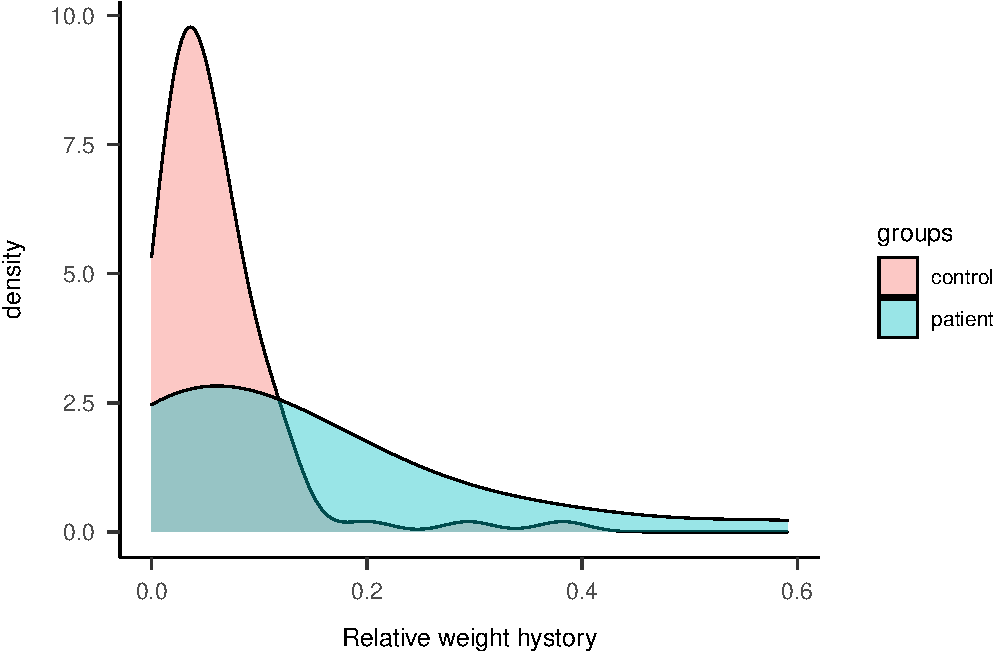
\includegraphics{046_weight_history_alpha_files/figure-latex/unnamed-chunk-4-1.pdf}

Split participants in patients, at-risk, and control

\begin{Shaded}
\begin{Highlighting}[]
\NormalTok{dd}\SpecialCharTok{$}\NormalTok{Group }\OtherTok{\textless{}{-}} \FunctionTok{factor}\NormalTok{(}
  \FunctionTok{ifelse}\NormalTok{(dd}\SpecialCharTok{$}\NormalTok{group }\SpecialCharTok{==} \DecValTok{0}\NormalTok{, }\StringTok{"control"}\NormalTok{, }\FunctionTok{ifelse}\NormalTok{(dd}\SpecialCharTok{$}\NormalTok{group }\SpecialCharTok{==} \DecValTok{1}\NormalTok{, }\StringTok{"at risk"}\NormalTok{, }\StringTok{"patient"}\NormalTok{)))}

\NormalTok{foo }\OtherTok{\textless{}{-}}\NormalTok{ dd[}\SpecialCharTok{!}\FunctionTok{is.na}\NormalTok{(dd}\SpecialCharTok{$}\NormalTok{Group), ]}
\FunctionTok{table}\NormalTok{(foo}\SpecialCharTok{$}\NormalTok{Group)}
\end{Highlighting}
\end{Shaded}

\begin{verbatim}
## 
## at risk control patient 
##      12      68      37
\end{verbatim}

\begin{verbatim}
## Warning: Removed 16 rows containing non-finite values (stat_density).
\end{verbatim}

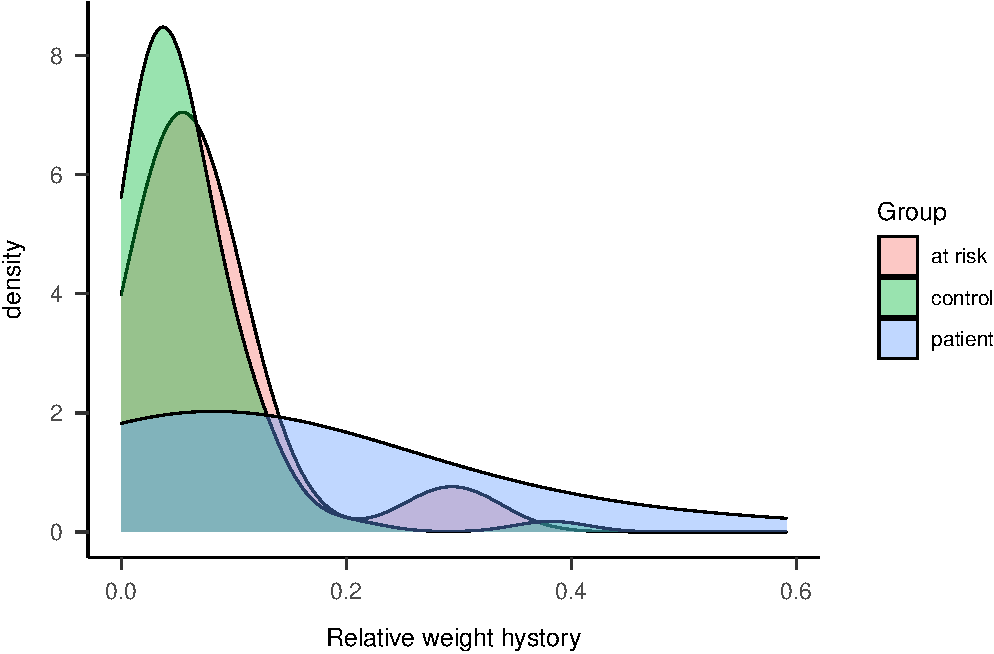
\includegraphics{046_weight_history_alpha_files/figure-latex/unnamed-chunk-6-1.pdf}

The at-risk group is very similar to the control group, and both differs
from the patient group.

\begin{Shaded}
\begin{Highlighting}[]
\CommentTok{\# Compute BMI}
\NormalTok{foo}\SpecialCharTok{$}\NormalTok{BMI }\OtherTok{\textless{}{-}}\NormalTok{ foo}\SpecialCharTok{$}\NormalTok{present\_weight }\SpecialCharTok{/}\NormalTok{ (foo}\SpecialCharTok{$}\NormalTok{height}\SpecialCharTok{/}\DecValTok{100}\NormalTok{)}\SpecialCharTok{\^{}}\DecValTok{2}
\NormalTok{foo}\SpecialCharTok{$}\NormalTok{bmi }\OtherTok{\textless{}{-}} \FunctionTok{as.numeric}\NormalTok{(}\FunctionTok{scale}\NormalTok{(foo}\SpecialCharTok{$}\NormalTok{BMI))}
\end{Highlighting}
\end{Shaded}

\begin{verbatim}
## Warning: Removed 16 rows containing non-finite values (stat_density).
\end{verbatim}

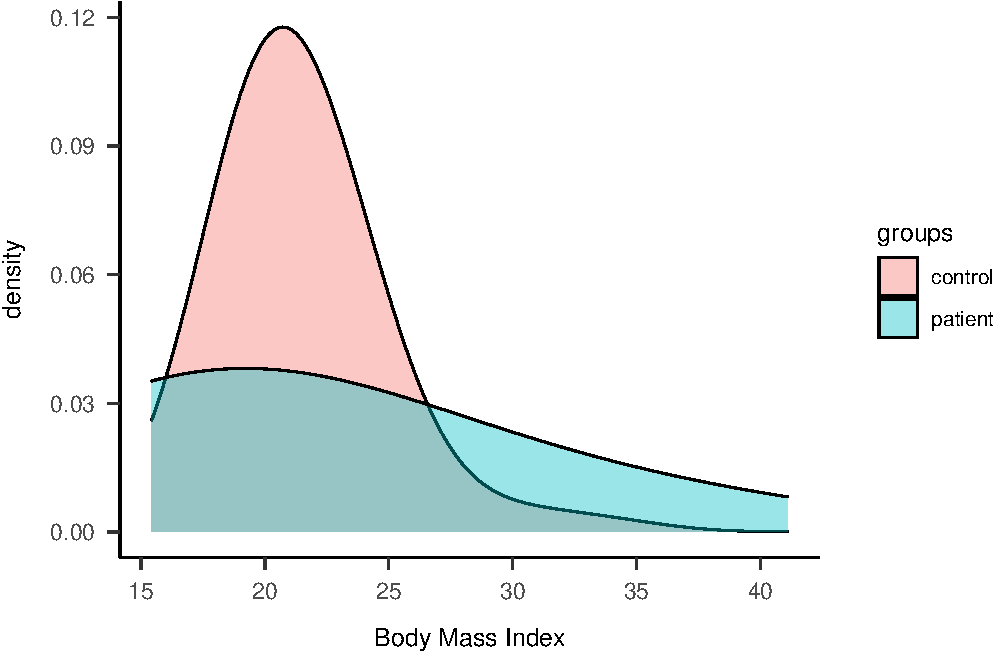
\includegraphics{046_weight_history_alpha_files/figure-latex/unnamed-chunk-8-1.pdf}

\begin{verbatim}
## Warning: Removed 16 rows containing non-finite values (stat_density).
\end{verbatim}

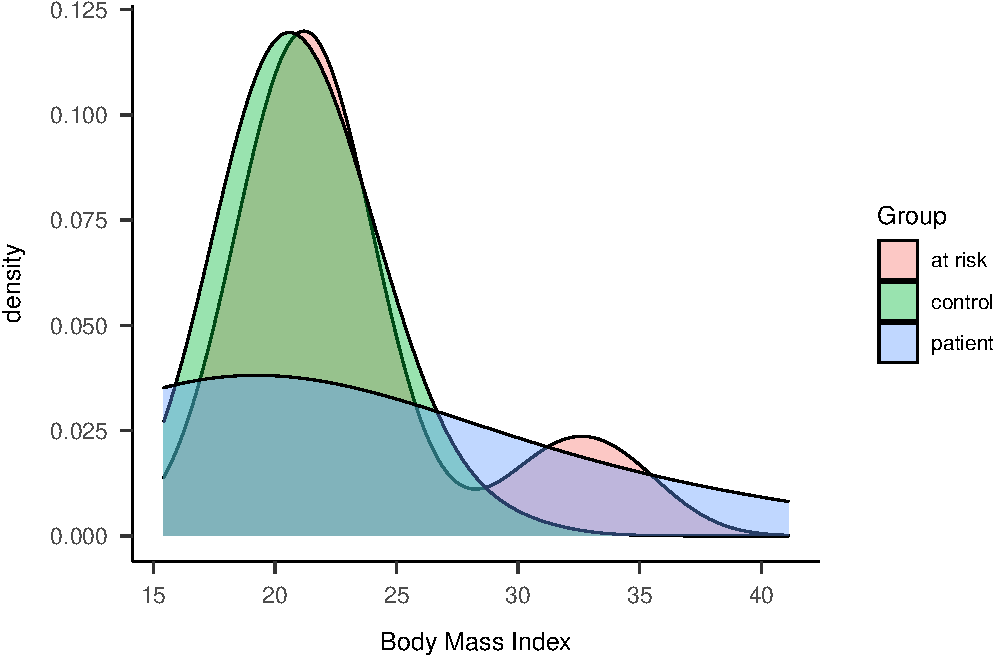
\includegraphics{046_weight_history_alpha_files/figure-latex/unnamed-chunk-9-1.pdf}

\begin{verbatim}
##         [,1] [,2]
## at risk    1    0
## control    0    1
## patient   -1   -1
\end{verbatim}

\begin{verbatim}
## Warning: Rows containing NAs were excluded from the model.
\end{verbatim}

\begin{verbatim}
## Start sampling
\end{verbatim}

\begin{verbatim}
## Running MCMC with 4 chains, at most 6 in parallel...
## 
## Chain 1 Iteration:    1 / 4000 [  0%]  (Warmup) 
## Chain 2 Iteration:    1 / 4000 [  0%]  (Warmup) 
## Chain 3 Iteration:    1 / 4000 [  0%]  (Warmup) 
## Chain 4 Iteration:    1 / 4000 [  0%]  (Warmup) 
## Chain 1 Iteration:  100 / 4000 [  2%]  (Warmup) 
## Chain 2 Iteration:  100 / 4000 [  2%]  (Warmup) 
## Chain 3 Iteration:  100 / 4000 [  2%]  (Warmup) 
## Chain 4 Iteration:  100 / 4000 [  2%]  (Warmup) 
## Chain 1 Iteration:  200 / 4000 [  5%]  (Warmup) 
## Chain 4 Iteration:  200 / 4000 [  5%]  (Warmup) 
## Chain 4 Iteration:  300 / 4000 [  7%]  (Warmup) 
## Chain 1 Iteration:  300 / 4000 [  7%]  (Warmup) 
## Chain 2 Iteration:  200 / 4000 [  5%]  (Warmup) 
## Chain 3 Iteration:  200 / 4000 [  5%]  (Warmup) 
## Chain 4 Iteration:  400 / 4000 [ 10%]  (Warmup) 
## Chain 1 Iteration:  400 / 4000 [ 10%]  (Warmup) 
## Chain 3 Iteration:  300 / 4000 [  7%]  (Warmup) 
## Chain 2 Iteration:  300 / 4000 [  7%]  (Warmup) 
## Chain 4 Iteration:  500 / 4000 [ 12%]  (Warmup) 
## Chain 1 Iteration:  500 / 4000 [ 12%]  (Warmup) 
## Chain 3 Iteration:  400 / 4000 [ 10%]  (Warmup) 
## Chain 4 Iteration:  600 / 4000 [ 15%]  (Warmup) 
## Chain 1 Iteration:  600 / 4000 [ 15%]  (Warmup) 
## Chain 2 Iteration:  400 / 4000 [ 10%]  (Warmup) 
## Chain 4 Iteration:  700 / 4000 [ 17%]  (Warmup) 
## Chain 1 Iteration:  700 / 4000 [ 17%]  (Warmup) 
## Chain 2 Iteration:  500 / 4000 [ 12%]  (Warmup) 
## Chain 3 Iteration:  500 / 4000 [ 12%]  (Warmup) 
## Chain 4 Iteration:  800 / 4000 [ 20%]  (Warmup) 
## Chain 2 Iteration:  600 / 4000 [ 15%]  (Warmup) 
## Chain 3 Iteration:  600 / 4000 [ 15%]  (Warmup) 
## Chain 1 Iteration:  800 / 4000 [ 20%]  (Warmup) 
## Chain 1 Iteration:  900 / 4000 [ 22%]  (Warmup) 
## Chain 2 Iteration:  700 / 4000 [ 17%]  (Warmup) 
## Chain 4 Iteration:  900 / 4000 [ 22%]  (Warmup) 
## Chain 3 Iteration:  700 / 4000 [ 17%]  (Warmup) 
## Chain 4 Iteration: 1000 / 4000 [ 25%]  (Warmup) 
## Chain 1 Iteration: 1000 / 4000 [ 25%]  (Warmup) 
## Chain 2 Iteration:  800 / 4000 [ 20%]  (Warmup) 
## Chain 3 Iteration:  800 / 4000 [ 20%]  (Warmup) 
## Chain 4 Iteration: 1100 / 4000 [ 27%]  (Warmup) 
## Chain 1 Iteration: 1100 / 4000 [ 27%]  (Warmup) 
## Chain 2 Iteration:  900 / 4000 [ 22%]  (Warmup) 
## Chain 1 Iteration: 1200 / 4000 [ 30%]  (Warmup) 
## Chain 2 Iteration: 1000 / 4000 [ 25%]  (Warmup) 
## Chain 3 Iteration:  900 / 4000 [ 22%]  (Warmup) 
## Chain 4 Iteration: 1200 / 4000 [ 30%]  (Warmup) 
## Chain 4 Iteration: 1300 / 4000 [ 32%]  (Warmup) 
## Chain 1 Iteration: 1300 / 4000 [ 32%]  (Warmup) 
## Chain 2 Iteration: 1100 / 4000 [ 27%]  (Warmup) 
## Chain 3 Iteration: 1000 / 4000 [ 25%]  (Warmup) 
## Chain 4 Iteration: 1400 / 4000 [ 35%]  (Warmup) 
## Chain 1 Iteration: 1400 / 4000 [ 35%]  (Warmup) 
## Chain 2 Iteration: 1200 / 4000 [ 30%]  (Warmup) 
## Chain 3 Iteration: 1100 / 4000 [ 27%]  (Warmup) 
## Chain 4 Iteration: 1500 / 4000 [ 37%]  (Warmup) 
## Chain 1 Iteration: 1500 / 4000 [ 37%]  (Warmup) 
## Chain 2 Iteration: 1300 / 4000 [ 32%]  (Warmup) 
## Chain 3 Iteration: 1200 / 4000 [ 30%]  (Warmup) 
## Chain 4 Iteration: 1600 / 4000 [ 40%]  (Warmup) 
## Chain 1 Iteration: 1600 / 4000 [ 40%]  (Warmup) 
## Chain 2 Iteration: 1400 / 4000 [ 35%]  (Warmup) 
## Chain 3 Iteration: 1300 / 4000 [ 32%]  (Warmup) 
## Chain 4 Iteration: 1700 / 4000 [ 42%]  (Warmup) 
## Chain 1 Iteration: 1700 / 4000 [ 42%]  (Warmup) 
## Chain 2 Iteration: 1500 / 4000 [ 37%]  (Warmup) 
## Chain 3 Iteration: 1400 / 4000 [ 35%]  (Warmup) 
## Chain 4 Iteration: 1800 / 4000 [ 45%]  (Warmup) 
## Chain 1 Iteration: 1800 / 4000 [ 45%]  (Warmup) 
## Chain 2 Iteration: 1600 / 4000 [ 40%]  (Warmup) 
## Chain 3 Iteration: 1500 / 4000 [ 37%]  (Warmup) 
## Chain 4 Iteration: 1900 / 4000 [ 47%]  (Warmup) 
## Chain 1 Iteration: 1900 / 4000 [ 47%]  (Warmup) 
## Chain 2 Iteration: 1700 / 4000 [ 42%]  (Warmup) 
## Chain 2 Iteration: 1800 / 4000 [ 45%]  (Warmup) 
## Chain 3 Iteration: 1600 / 4000 [ 40%]  (Warmup) 
## Chain 4 Iteration: 2000 / 4000 [ 50%]  (Warmup) 
## Chain 4 Iteration: 2001 / 4000 [ 50%]  (Sampling) 
## Chain 1 Iteration: 2000 / 4000 [ 50%]  (Warmup) 
## Chain 1 Iteration: 2001 / 4000 [ 50%]  (Sampling) 
## Chain 4 Iteration: 2100 / 4000 [ 52%]  (Sampling) 
## Chain 2 Iteration: 1900 / 4000 [ 47%]  (Warmup) 
## Chain 3 Iteration: 1700 / 4000 [ 42%]  (Warmup) 
## Chain 1 Iteration: 2100 / 4000 [ 52%]  (Sampling) 
## Chain 3 Iteration: 1800 / 4000 [ 45%]  (Warmup) 
## Chain 4 Iteration: 2200 / 4000 [ 55%]  (Sampling) 
## Chain 1 Iteration: 2200 / 4000 [ 55%]  (Sampling) 
## Chain 2 Iteration: 2000 / 4000 [ 50%]  (Warmup) 
## Chain 2 Iteration: 2001 / 4000 [ 50%]  (Sampling) 
## Chain 3 Iteration: 1900 / 4000 [ 47%]  (Warmup) 
## Chain 4 Iteration: 2300 / 4000 [ 57%]  (Sampling) 
## Chain 4 Iteration: 2400 / 4000 [ 60%]  (Sampling) 
## Chain 2 Iteration: 2100 / 4000 [ 52%]  (Sampling) 
## Chain 1 Iteration: 2300 / 4000 [ 57%]  (Sampling) 
## Chain 4 Iteration: 2500 / 4000 [ 62%]  (Sampling) 
## Chain 2 Iteration: 2200 / 4000 [ 55%]  (Sampling) 
## Chain 3 Iteration: 2000 / 4000 [ 50%]  (Warmup) 
## Chain 3 Iteration: 2001 / 4000 [ 50%]  (Sampling) 
## Chain 1 Iteration: 2400 / 4000 [ 60%]  (Sampling) 
## Chain 4 Iteration: 2600 / 4000 [ 65%]  (Sampling) 
## Chain 2 Iteration: 2300 / 4000 [ 57%]  (Sampling) 
## Chain 3 Iteration: 2100 / 4000 [ 52%]  (Sampling) 
## Chain 4 Iteration: 2700 / 4000 [ 67%]  (Sampling) 
## Chain 1 Iteration: 2500 / 4000 [ 62%]  (Sampling) 
## Chain 2 Iteration: 2400 / 4000 [ 60%]  (Sampling) 
## Chain 3 Iteration: 2200 / 4000 [ 55%]  (Sampling) 
## Chain 4 Iteration: 2800 / 4000 [ 70%]  (Sampling) 
## Chain 1 Iteration: 2600 / 4000 [ 65%]  (Sampling) 
## Chain 2 Iteration: 2500 / 4000 [ 62%]  (Sampling) 
## Chain 3 Iteration: 2300 / 4000 [ 57%]  (Sampling) 
## Chain 4 Iteration: 2900 / 4000 [ 72%]  (Sampling) 
## Chain 1 Iteration: 2700 / 4000 [ 67%]  (Sampling) 
## Chain 4 Iteration: 3000 / 4000 [ 75%]  (Sampling) 
## Chain 2 Iteration: 2600 / 4000 [ 65%]  (Sampling) 
## Chain 3 Iteration: 2400 / 4000 [ 60%]  (Sampling) 
## Chain 1 Iteration: 2800 / 4000 [ 70%]  (Sampling) 
## Chain 4 Iteration: 3100 / 4000 [ 77%]  (Sampling) 
## Chain 2 Iteration: 2700 / 4000 [ 67%]  (Sampling) 
## Chain 3 Iteration: 2500 / 4000 [ 62%]  (Sampling) 
## Chain 1 Iteration: 2900 / 4000 [ 72%]  (Sampling) 
## Chain 4 Iteration: 3200 / 4000 [ 80%]  (Sampling) 
## Chain 2 Iteration: 2800 / 4000 [ 70%]  (Sampling) 
## Chain 3 Iteration: 2600 / 4000 [ 65%]  (Sampling) 
## Chain 4 Iteration: 3300 / 4000 [ 82%]  (Sampling) 
## Chain 1 Iteration: 3000 / 4000 [ 75%]  (Sampling) 
## Chain 4 Iteration: 3400 / 4000 [ 85%]  (Sampling) 
## Chain 1 Iteration: 3100 / 4000 [ 77%]  (Sampling) 
## Chain 2 Iteration: 2900 / 4000 [ 72%]  (Sampling) 
## Chain 3 Iteration: 2700 / 4000 [ 67%]  (Sampling) 
## Chain 4 Iteration: 3500 / 4000 [ 87%]  (Sampling) 
## Chain 1 Iteration: 3200 / 4000 [ 80%]  (Sampling) 
## Chain 2 Iteration: 3000 / 4000 [ 75%]  (Sampling) 
## Chain 3 Iteration: 2800 / 4000 [ 70%]  (Sampling) 
## Chain 4 Iteration: 3600 / 4000 [ 90%]  (Sampling) 
## Chain 2 Iteration: 3100 / 4000 [ 77%]  (Sampling) 
## Chain 1 Iteration: 3300 / 4000 [ 82%]  (Sampling) 
## Chain 3 Iteration: 2900 / 4000 [ 72%]  (Sampling) 
## Chain 4 Iteration: 3700 / 4000 [ 92%]  (Sampling) 
## Chain 2 Iteration: 3200 / 4000 [ 80%]  (Sampling) 
## Chain 4 Iteration: 3800 / 4000 [ 95%]  (Sampling) 
## Chain 1 Iteration: 3400 / 4000 [ 85%]  (Sampling) 
## Chain 3 Iteration: 3000 / 4000 [ 75%]  (Sampling) 
## Chain 4 Iteration: 3900 / 4000 [ 97%]  (Sampling) 
## Chain 1 Iteration: 3500 / 4000 [ 87%]  (Sampling) 
## Chain 2 Iteration: 3300 / 4000 [ 82%]  (Sampling) 
## Chain 4 Iteration: 4000 / 4000 [100%]  (Sampling) 
## Chain 4 finished in 6.9 seconds.
## Chain 3 Iteration: 3100 / 4000 [ 77%]  (Sampling) 
## Chain 1 Iteration: 3600 / 4000 [ 90%]  (Sampling) 
## Chain 2 Iteration: 3400 / 4000 [ 85%]  (Sampling) 
## Chain 3 Iteration: 3200 / 4000 [ 80%]  (Sampling) 
## Chain 1 Iteration: 3700 / 4000 [ 92%]  (Sampling) 
## Chain 2 Iteration: 3500 / 4000 [ 87%]  (Sampling) 
## Chain 3 Iteration: 3300 / 4000 [ 82%]  (Sampling) 
## Chain 1 Iteration: 3800 / 4000 [ 95%]  (Sampling) 
## Chain 2 Iteration: 3600 / 4000 [ 90%]  (Sampling) 
## Chain 3 Iteration: 3400 / 4000 [ 85%]  (Sampling) 
## Chain 1 Iteration: 3900 / 4000 [ 97%]  (Sampling) 
## Chain 2 Iteration: 3700 / 4000 [ 92%]  (Sampling) 
## Chain 3 Iteration: 3500 / 4000 [ 87%]  (Sampling) 
## Chain 1 Iteration: 4000 / 4000 [100%]  (Sampling) 
## Chain 2 Iteration: 3800 / 4000 [ 95%]  (Sampling) 
## Chain 1 finished in 7.9 seconds.
## Chain 2 Iteration: 3900 / 4000 [ 97%]  (Sampling) 
## Chain 3 Iteration: 3600 / 4000 [ 90%]  (Sampling) 
## Chain 2 Iteration: 4000 / 4000 [100%]  (Sampling) 
## Chain 3 Iteration: 3700 / 4000 [ 92%]  (Sampling) 
## Chain 2 finished in 8.3 seconds.
## Chain 3 Iteration: 3800 / 4000 [ 95%]  (Sampling) 
## Chain 3 Iteration: 3900 / 4000 [ 97%]  (Sampling) 
## Chain 3 Iteration: 4000 / 4000 [100%]  (Sampling) 
## Chain 3 finished in 9.0 seconds.
## 
## All 4 chains finished successfully.
## Mean chain execution time: 8.1 seconds.
## Total execution time: 9.3 seconds.
\end{verbatim}

\begin{verbatim}
##  Family: zero_inflated_beta 
##   Links: mu = logit; phi = identity; zi = identity 
## Formula: rws ~ Group + bmi + (a_neither + v_food + v_social + t_food + t_social + z_food + z_social + alpha_neg_food + alpha_neg_social + alpha_pos_food + alpha_pos_social + oral_control + dieting + bulimia + bsq14_tot + ros_tot + sias + mps_ps + mps_o + mps_cmd + mps_pepc + orto_tot) 
##    Data: foo (Number of observations: 95) 
## Samples: 4 chains, each with iter = 4000; warmup = 2000; thin = 1;
##          total post-warmup samples = 8000
## 
## Population-Level Effects: 
##                  Estimate Est.Error l-95% CI u-95% CI Rhat Bulk_ESS Tail_ESS
## Intercept           -2.78      0.17    -3.14    -2.46 1.00     3791     4311
## Group1              -0.44      0.25    -0.95     0.04 1.00     3511     4235
## Group2               0.29      0.25    -0.18     0.81 1.00     4076     4776
## bmi                  0.17      0.13    -0.10     0.42 1.00     4484     5378
## a_neither           -0.10      0.10    -0.29     0.10 1.00     5768     5974
## v_food               0.15      0.21    -0.27     0.56 1.00     4009     5284
## v_social            -0.13      0.12    -0.37     0.11 1.00     5296     5742
## t_food              -0.30      0.16    -0.62     0.01 1.00     3660     4766
## t_social             0.27      0.15    -0.03     0.56 1.00     4246     5353
## z_food              -0.04      0.11    -0.26     0.18 1.00     5738     5902
## z_social             0.03      0.08    -0.13     0.21 1.00     6917     5742
## alpha_neg_food      -0.06      0.12    -0.29     0.18 1.00     5433     5930
## alpha_neg_social     0.26      0.11     0.05     0.47 1.00     6993     6123
## alpha_pos_food       0.04      0.12    -0.20     0.28 1.00     4816     5925
## alpha_pos_social     0.23      0.11     0.02     0.44 1.00     6281     6322
## oral_control         0.47      0.14     0.20     0.75 1.00     7231     5934
## dieting              0.51      0.23     0.08     0.98 1.00     3903     4539
## bulimia              0.03      0.20    -0.35     0.42 1.00     5246     5992
## bsq14_tot            0.03      0.21    -0.38     0.44 1.00     4497     5186
## ros_tot              0.01      0.19    -0.35     0.38 1.00     5521     6101
## sias                -0.28      0.15    -0.56     0.01 1.00     4840     5692
## mps_ps               0.06      0.11    -0.16     0.28 1.00     5865     5406
## mps_o               -0.06      0.10    -0.24     0.13 1.00     6972     5597
## mps_cmd             -0.05      0.20    -0.44     0.35 1.00     4537     5137
## mps_pepc             0.02      0.13    -0.25     0.27 1.00     4883     5889
## orto_tot             0.19      0.15    -0.10     0.49 1.00     5677     6195
## 
## Family Specific Parameters: 
##     Estimate Est.Error l-95% CI u-95% CI Rhat Bulk_ESS Tail_ESS
## phi    26.41      4.60    18.31    36.38 1.00     6353     5777
## zi      0.07      0.03     0.03     0.13 1.00    11762     5047
## 
## Samples were drawn using sample(hmc). For each parameter, Bulk_ESS
## and Tail_ESS are effective sample size measures, and Rhat is the potential
## scale reduction factor on split chains (at convergence, Rhat = 1).
\end{verbatim}

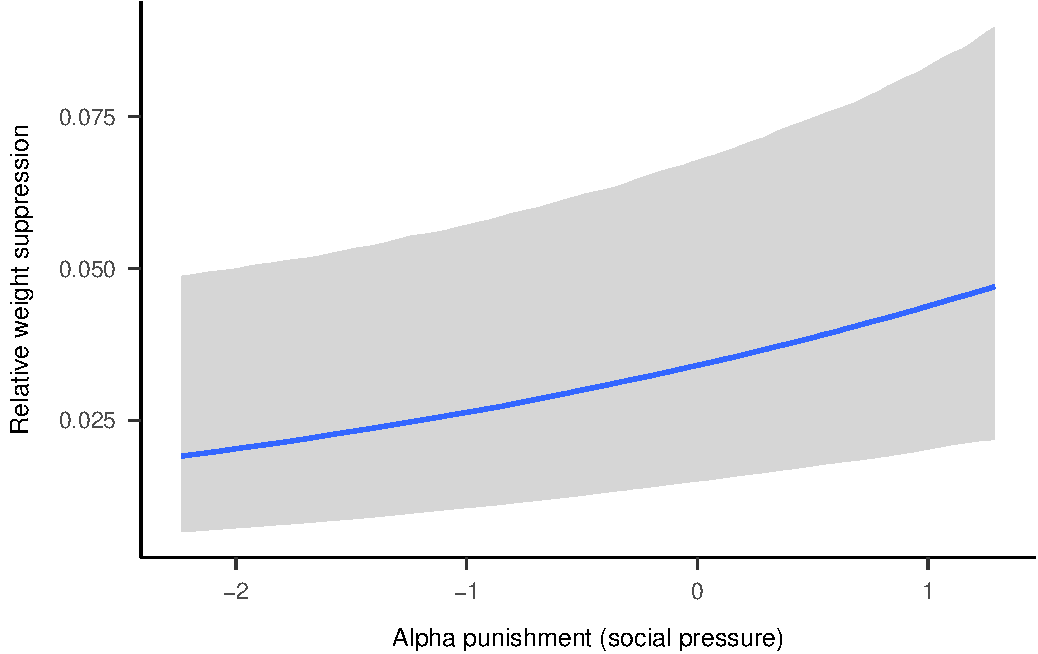
\includegraphics{046_weight_history_alpha_files/figure-latex/unnamed-chunk-9-2.pdf}
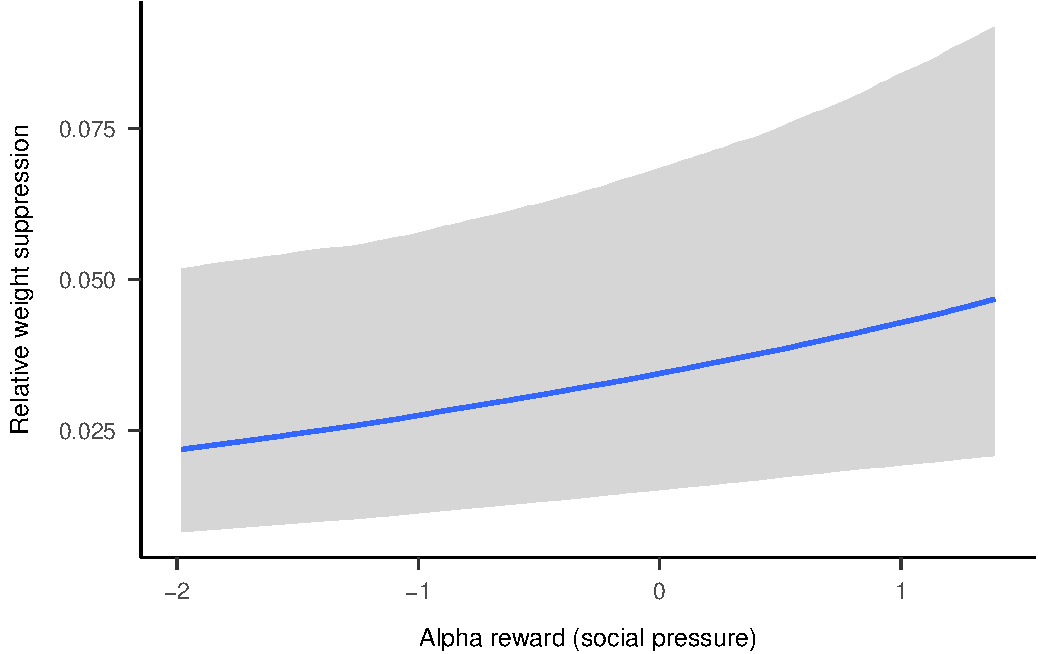
\includegraphics{046_weight_history_alpha_files/figure-latex/unnamed-chunk-9-3.pdf}
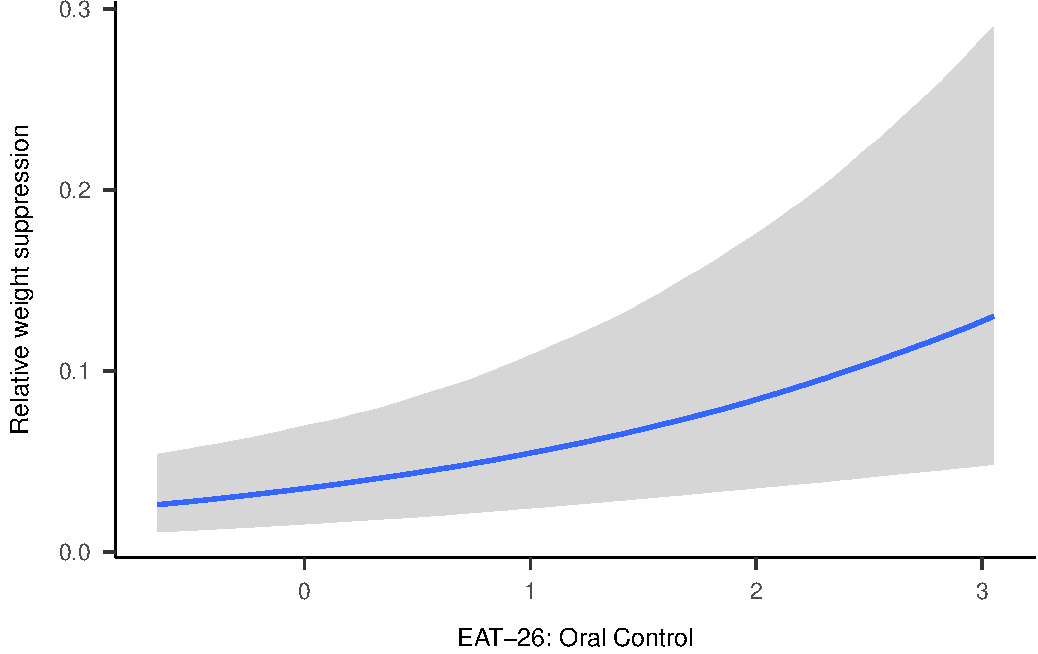
\includegraphics{046_weight_history_alpha_files/figure-latex/unnamed-chunk-9-4.pdf}
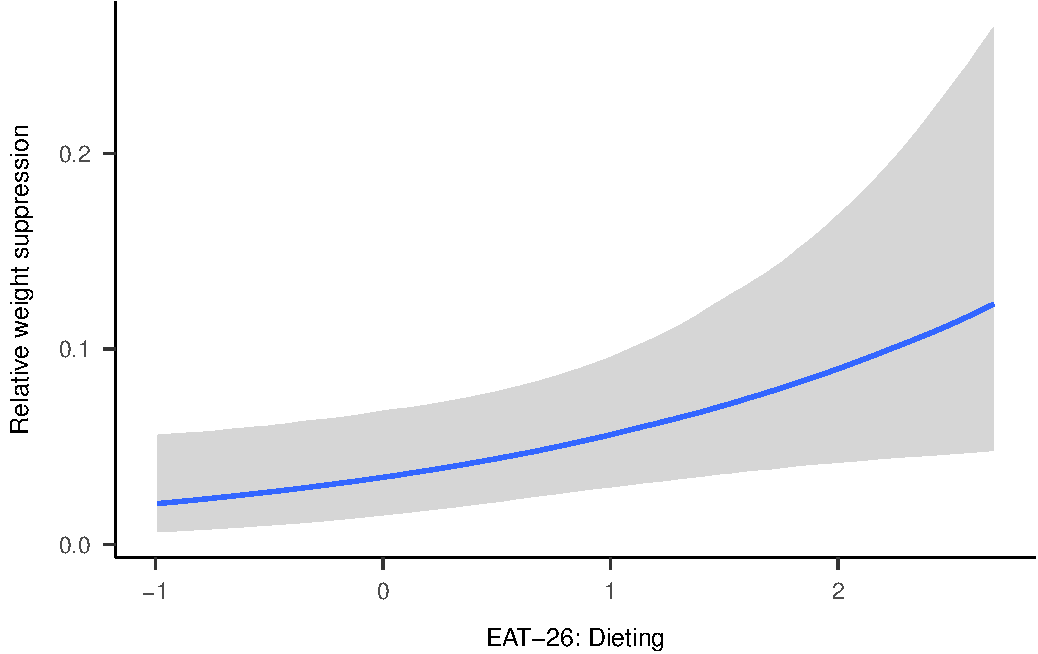
\includegraphics{046_weight_history_alpha_files/figure-latex/unnamed-chunk-9-5.pdf}

\begin{verbatim}
## Sampling priors, please wait...
\end{verbatim}

\begin{verbatim}
## Caricamento dei namespace richiesti: logspline
\end{verbatim}

\begin{verbatim}
## Bayes Factor (Savage-Dickey density ratio)
## 
## Parameter        |       BF
## ---------------------------
## (Intercept)      | 0.00e+00
## Group1           |    0.040
## Group2           |    0.395
## bmi              |    0.271
## a_neither        |    0.026
## v_food           |    0.213
## v_social         |    0.030
## t_food           |    0.028
## t_social         |    0.649
## z_food           |    0.042
## z_social         |    0.061
## alpha_neg_food   |    0.044
## alpha_neg_social |     2.12
## alpha_pos_food   |    0.082
## alpha_pos_social |     1.01
## oral_control     |    24.61
## dieting          |     3.23
## bulimia          |    0.115
## bsq14_tot        |    0.127
## ros_tot          |    0.103
## sias             |    0.026
## mps_ps           |    0.089
## mps_o            |    0.033
## mps_cmd          |    0.080
## mps_pepc         |    0.075
## orto_tot         |    0.287
## 
## * Evidence Against The Null: 0
## *                 Direction: Right-Sided test
\end{verbatim}

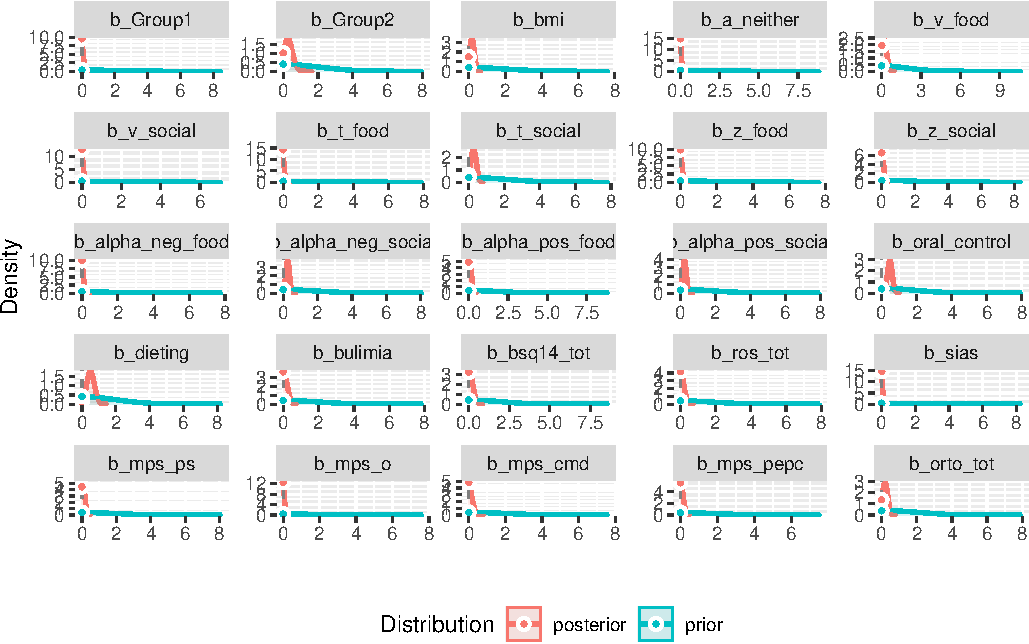
\includegraphics{046_weight_history_alpha_files/figure-latex/unnamed-chunk-9-6.pdf}

Marginal effects

Alpha punishment is not a robust effect. Alpha reward

\begin{Shaded}
\begin{Highlighting}[]
\NormalTok{m10 }\OtherTok{\textless{}{-}} \FunctionTok{brm}\NormalTok{(}
\NormalTok{  rws }\SpecialCharTok{\textasciitilde{}}\NormalTok{ alpha\_pos\_social,}
  \AttributeTok{data =}\NormalTok{ foo, }
  \AttributeTok{prior =}\NormalTok{ prior\_ma,}
  \AttributeTok{family =} \FunctionTok{zero\_inflated\_beta}\NormalTok{(),}
  \AttributeTok{control =} \FunctionTok{list}\NormalTok{(}\AttributeTok{adapt\_delta =} \FloatTok{0.98}\NormalTok{),}
  \AttributeTok{iter =} \DecValTok{4000}\NormalTok{,}
  \AttributeTok{cores =} \DecValTok{6}\NormalTok{,}
  \AttributeTok{backend =} \StringTok{"cmdstan"}
\NormalTok{)}
\end{Highlighting}
\end{Shaded}

\begin{verbatim}
## Warning: Rows containing NAs were excluded from the model.
\end{verbatim}

\begin{verbatim}
## Start sampling
\end{verbatim}

\begin{verbatim}
## Running MCMC with 4 chains, at most 6 in parallel...
## 
## Chain 1 Iteration:    1 / 4000 [  0%]  (Warmup) 
## Chain 1 Iteration:  100 / 4000 [  2%]  (Warmup) 
## Chain 1 Iteration:  200 / 4000 [  5%]  (Warmup) 
## Chain 1 Iteration:  300 / 4000 [  7%]  (Warmup) 
## Chain 1 Iteration:  400 / 4000 [ 10%]  (Warmup) 
## Chain 2 Iteration:    1 / 4000 [  0%]  (Warmup) 
## Chain 2 Iteration:  100 / 4000 [  2%]  (Warmup) 
## Chain 2 Iteration:  200 / 4000 [  5%]  (Warmup) 
## Chain 3 Iteration:    1 / 4000 [  0%]  (Warmup) 
## Chain 3 Iteration:  100 / 4000 [  2%]  (Warmup) 
## Chain 3 Iteration:  200 / 4000 [  5%]  (Warmup) 
## Chain 4 Iteration:    1 / 4000 [  0%]  (Warmup) 
## Chain 4 Iteration:  100 / 4000 [  2%]  (Warmup) 
## Chain 4 Iteration:  200 / 4000 [  5%]  (Warmup) 
## Chain 4 Iteration:  300 / 4000 [  7%]  (Warmup) 
## Chain 1 Iteration:  500 / 4000 [ 12%]  (Warmup) 
## Chain 1 Iteration:  600 / 4000 [ 15%]  (Warmup) 
## Chain 1 Iteration:  700 / 4000 [ 17%]  (Warmup) 
## Chain 1 Iteration:  800 / 4000 [ 20%]  (Warmup) 
## Chain 2 Iteration:  300 / 4000 [  7%]  (Warmup) 
## Chain 2 Iteration:  400 / 4000 [ 10%]  (Warmup) 
## Chain 2 Iteration:  500 / 4000 [ 12%]  (Warmup) 
## Chain 2 Iteration:  600 / 4000 [ 15%]  (Warmup) 
## Chain 3 Iteration:  300 / 4000 [  7%]  (Warmup) 
## Chain 3 Iteration:  400 / 4000 [ 10%]  (Warmup) 
## Chain 3 Iteration:  500 / 4000 [ 12%]  (Warmup) 
## Chain 4 Iteration:  400 / 4000 [ 10%]  (Warmup) 
## Chain 4 Iteration:  500 / 4000 [ 12%]  (Warmup) 
## Chain 4 Iteration:  600 / 4000 [ 15%]  (Warmup) 
## Chain 4 Iteration:  700 / 4000 [ 17%]  (Warmup) 
## Chain 1 Iteration:  900 / 4000 [ 22%]  (Warmup) 
## Chain 1 Iteration: 1000 / 4000 [ 25%]  (Warmup) 
## Chain 1 Iteration: 1100 / 4000 [ 27%]  (Warmup) 
## Chain 1 Iteration: 1200 / 4000 [ 30%]  (Warmup) 
## Chain 2 Iteration:  700 / 4000 [ 17%]  (Warmup) 
## Chain 2 Iteration:  800 / 4000 [ 20%]  (Warmup) 
## Chain 2 Iteration:  900 / 4000 [ 22%]  (Warmup) 
## Chain 2 Iteration: 1000 / 4000 [ 25%]  (Warmup) 
## Chain 3 Iteration:  600 / 4000 [ 15%]  (Warmup) 
## Chain 3 Iteration:  700 / 4000 [ 17%]  (Warmup) 
## Chain 3 Iteration:  800 / 4000 [ 20%]  (Warmup) 
## Chain 4 Iteration:  800 / 4000 [ 20%]  (Warmup) 
## Chain 4 Iteration:  900 / 4000 [ 22%]  (Warmup) 
## Chain 4 Iteration: 1000 / 4000 [ 25%]  (Warmup) 
## Chain 1 Iteration: 1300 / 4000 [ 32%]  (Warmup) 
## Chain 1 Iteration: 1400 / 4000 [ 35%]  (Warmup) 
## Chain 1 Iteration: 1500 / 4000 [ 37%]  (Warmup) 
## Chain 2 Iteration: 1100 / 4000 [ 27%]  (Warmup) 
## Chain 2 Iteration: 1200 / 4000 [ 30%]  (Warmup) 
## Chain 2 Iteration: 1300 / 4000 [ 32%]  (Warmup) 
## Chain 3 Iteration:  900 / 4000 [ 22%]  (Warmup) 
## Chain 3 Iteration: 1000 / 4000 [ 25%]  (Warmup) 
## Chain 3 Iteration: 1100 / 4000 [ 27%]  (Warmup) 
## Chain 4 Iteration: 1100 / 4000 [ 27%]  (Warmup) 
## Chain 4 Iteration: 1200 / 4000 [ 30%]  (Warmup) 
## Chain 4 Iteration: 1300 / 4000 [ 32%]  (Warmup) 
## Chain 1 Iteration: 1600 / 4000 [ 40%]  (Warmup) 
## Chain 1 Iteration: 1700 / 4000 [ 42%]  (Warmup) 
## Chain 1 Iteration: 1800 / 4000 [ 45%]  (Warmup) 
## Chain 2 Iteration: 1400 / 4000 [ 35%]  (Warmup) 
## Chain 2 Iteration: 1500 / 4000 [ 37%]  (Warmup) 
## Chain 2 Iteration: 1600 / 4000 [ 40%]  (Warmup) 
## Chain 2 Iteration: 1700 / 4000 [ 42%]  (Warmup) 
## Chain 3 Iteration: 1200 / 4000 [ 30%]  (Warmup) 
## Chain 3 Iteration: 1300 / 4000 [ 32%]  (Warmup) 
## Chain 3 Iteration: 1400 / 4000 [ 35%]  (Warmup) 
## Chain 3 Iteration: 1500 / 4000 [ 37%]  (Warmup) 
## Chain 4 Iteration: 1400 / 4000 [ 35%]  (Warmup) 
## Chain 4 Iteration: 1500 / 4000 [ 37%]  (Warmup) 
## Chain 4 Iteration: 1600 / 4000 [ 40%]  (Warmup) 
## Chain 4 Iteration: 1700 / 4000 [ 42%]  (Warmup) 
## Chain 1 Iteration: 1900 / 4000 [ 47%]  (Warmup) 
## Chain 1 Iteration: 2000 / 4000 [ 50%]  (Warmup) 
## Chain 1 Iteration: 2001 / 4000 [ 50%]  (Sampling) 
## Chain 1 Iteration: 2100 / 4000 [ 52%]  (Sampling) 
## Chain 2 Iteration: 1800 / 4000 [ 45%]  (Warmup) 
## Chain 2 Iteration: 1900 / 4000 [ 47%]  (Warmup) 
## Chain 2 Iteration: 2000 / 4000 [ 50%]  (Warmup) 
## Chain 2 Iteration: 2001 / 4000 [ 50%]  (Sampling) 
## Chain 3 Iteration: 1600 / 4000 [ 40%]  (Warmup) 
## Chain 3 Iteration: 1700 / 4000 [ 42%]  (Warmup) 
## Chain 3 Iteration: 1800 / 4000 [ 45%]  (Warmup) 
## Chain 3 Iteration: 1900 / 4000 [ 47%]  (Warmup) 
## Chain 4 Iteration: 1800 / 4000 [ 45%]  (Warmup) 
## Chain 4 Iteration: 1900 / 4000 [ 47%]  (Warmup) 
## Chain 4 Iteration: 2000 / 4000 [ 50%]  (Warmup) 
## Chain 4 Iteration: 2001 / 4000 [ 50%]  (Sampling) 
## Chain 1 Iteration: 2200 / 4000 [ 55%]  (Sampling) 
## Chain 1 Iteration: 2300 / 4000 [ 57%]  (Sampling) 
## Chain 1 Iteration: 2400 / 4000 [ 60%]  (Sampling) 
## Chain 2 Iteration: 2100 / 4000 [ 52%]  (Sampling) 
## Chain 2 Iteration: 2200 / 4000 [ 55%]  (Sampling) 
## Chain 3 Iteration: 2000 / 4000 [ 50%]  (Warmup) 
## Chain 3 Iteration: 2001 / 4000 [ 50%]  (Sampling) 
## Chain 3 Iteration: 2100 / 4000 [ 52%]  (Sampling) 
## Chain 4 Iteration: 2100 / 4000 [ 52%]  (Sampling) 
## Chain 4 Iteration: 2200 / 4000 [ 55%]  (Sampling) 
## Chain 4 Iteration: 2300 / 4000 [ 57%]  (Sampling) 
## Chain 1 Iteration: 2500 / 4000 [ 62%]  (Sampling) 
## Chain 1 Iteration: 2600 / 4000 [ 65%]  (Sampling) 
## Chain 1 Iteration: 2700 / 4000 [ 67%]  (Sampling) 
## Chain 2 Iteration: 2300 / 4000 [ 57%]  (Sampling) 
## Chain 2 Iteration: 2400 / 4000 [ 60%]  (Sampling) 
## Chain 2 Iteration: 2500 / 4000 [ 62%]  (Sampling) 
## Chain 3 Iteration: 2200 / 4000 [ 55%]  (Sampling) 
## Chain 3 Iteration: 2300 / 4000 [ 57%]  (Sampling) 
## Chain 3 Iteration: 2400 / 4000 [ 60%]  (Sampling) 
## Chain 4 Iteration: 2400 / 4000 [ 60%]  (Sampling) 
## Chain 4 Iteration: 2500 / 4000 [ 62%]  (Sampling) 
## Chain 4 Iteration: 2600 / 4000 [ 65%]  (Sampling) 
## Chain 1 Iteration: 2800 / 4000 [ 70%]  (Sampling) 
## Chain 1 Iteration: 2900 / 4000 [ 72%]  (Sampling) 
## Chain 1 Iteration: 3000 / 4000 [ 75%]  (Sampling) 
## Chain 2 Iteration: 2600 / 4000 [ 65%]  (Sampling) 
## Chain 2 Iteration: 2700 / 4000 [ 67%]  (Sampling) 
## Chain 2 Iteration: 2800 / 4000 [ 70%]  (Sampling) 
## Chain 3 Iteration: 2500 / 4000 [ 62%]  (Sampling) 
## Chain 3 Iteration: 2600 / 4000 [ 65%]  (Sampling) 
## Chain 3 Iteration: 2700 / 4000 [ 67%]  (Sampling) 
## Chain 4 Iteration: 2700 / 4000 [ 67%]  (Sampling) 
## Chain 4 Iteration: 2800 / 4000 [ 70%]  (Sampling) 
## Chain 4 Iteration: 2900 / 4000 [ 72%]  (Sampling) 
## Chain 1 Iteration: 3100 / 4000 [ 77%]  (Sampling) 
## Chain 1 Iteration: 3200 / 4000 [ 80%]  (Sampling) 
## Chain 2 Iteration: 2900 / 4000 [ 72%]  (Sampling) 
## Chain 2 Iteration: 3000 / 4000 [ 75%]  (Sampling) 
## Chain 2 Iteration: 3100 / 4000 [ 77%]  (Sampling) 
## Chain 3 Iteration: 2800 / 4000 [ 70%]  (Sampling) 
## Chain 3 Iteration: 2900 / 4000 [ 72%]  (Sampling) 
## Chain 3 Iteration: 3000 / 4000 [ 75%]  (Sampling) 
## Chain 4 Iteration: 3000 / 4000 [ 75%]  (Sampling) 
## Chain 4 Iteration: 3100 / 4000 [ 77%]  (Sampling) 
## Chain 4 Iteration: 3200 / 4000 [ 80%]  (Sampling) 
## Chain 1 Iteration: 3300 / 4000 [ 82%]  (Sampling) 
## Chain 1 Iteration: 3400 / 4000 [ 85%]  (Sampling) 
## Chain 1 Iteration: 3500 / 4000 [ 87%]  (Sampling) 
## Chain 2 Iteration: 3200 / 4000 [ 80%]  (Sampling) 
## Chain 2 Iteration: 3300 / 4000 [ 82%]  (Sampling) 
## Chain 2 Iteration: 3400 / 4000 [ 85%]  (Sampling) 
## Chain 3 Iteration: 3100 / 4000 [ 77%]  (Sampling) 
## Chain 3 Iteration: 3200 / 4000 [ 80%]  (Sampling) 
## Chain 3 Iteration: 3300 / 4000 [ 82%]  (Sampling) 
## Chain 3 Iteration: 3400 / 4000 [ 85%]  (Sampling) 
## Chain 4 Iteration: 3300 / 4000 [ 82%]  (Sampling) 
## Chain 4 Iteration: 3400 / 4000 [ 85%]  (Sampling) 
## Chain 4 Iteration: 3500 / 4000 [ 87%]  (Sampling) 
## Chain 1 Iteration: 3600 / 4000 [ 90%]  (Sampling) 
## Chain 1 Iteration: 3700 / 4000 [ 92%]  (Sampling) 
## Chain 1 Iteration: 3800 / 4000 [ 95%]  (Sampling) 
## Chain 2 Iteration: 3500 / 4000 [ 87%]  (Sampling) 
## Chain 2 Iteration: 3600 / 4000 [ 90%]  (Sampling) 
## Chain 2 Iteration: 3700 / 4000 [ 92%]  (Sampling) 
## Chain 3 Iteration: 3500 / 4000 [ 87%]  (Sampling) 
## Chain 3 Iteration: 3600 / 4000 [ 90%]  (Sampling) 
## Chain 3 Iteration: 3700 / 4000 [ 92%]  (Sampling) 
## Chain 4 Iteration: 3600 / 4000 [ 90%]  (Sampling) 
## Chain 4 Iteration: 3700 / 4000 [ 92%]  (Sampling) 
## Chain 4 Iteration: 3800 / 4000 [ 95%]  (Sampling) 
## Chain 1 Iteration: 3900 / 4000 [ 97%]  (Sampling) 
## Chain 1 Iteration: 4000 / 4000 [100%]  (Sampling) 
## Chain 2 Iteration: 3800 / 4000 [ 95%]  (Sampling) 
## Chain 2 Iteration: 3900 / 4000 [ 97%]  (Sampling) 
## Chain 2 Iteration: 4000 / 4000 [100%]  (Sampling) 
## Chain 3 Iteration: 3800 / 4000 [ 95%]  (Sampling) 
## Chain 3 Iteration: 3900 / 4000 [ 97%]  (Sampling) 
## Chain 3 Iteration: 4000 / 4000 [100%]  (Sampling) 
## Chain 4 Iteration: 3900 / 4000 [ 97%]  (Sampling) 
## Chain 4 Iteration: 4000 / 4000 [100%]  (Sampling) 
## Chain 1 finished in 1.4 seconds.
## Chain 2 finished in 1.4 seconds.
## Chain 3 finished in 1.4 seconds.
## Chain 4 finished in 1.4 seconds.
## 
## All 4 chains finished successfully.
## Mean chain execution time: 1.4 seconds.
## Total execution time: 1.5 seconds.
\end{verbatim}

\begin{Shaded}
\begin{Highlighting}[]
\FunctionTok{summary}\NormalTok{(m10)}
\end{Highlighting}
\end{Shaded}

\begin{verbatim}
##  Family: zero_inflated_beta 
##   Links: mu = logit; phi = identity; zi = identity 
## Formula: rws ~ alpha_pos_social 
##    Data: foo (Number of observations: 98) 
## Samples: 4 chains, each with iter = 4000; warmup = 2000; thin = 1;
##          total post-warmup samples = 8000
## 
## Population-Level Effects: 
##                  Estimate Est.Error l-95% CI u-95% CI Rhat Bulk_ESS Tail_ESS
## Intercept           -2.43      0.10    -2.62    -2.24 1.00     5096     5323
## alpha_pos_social     0.19      0.08     0.04     0.34 1.00     6064     5075
## 
## Family Specific Parameters: 
##     Estimate Est.Error l-95% CI u-95% CI Rhat Bulk_ESS Tail_ESS
## phi    14.98      2.33    10.89    19.85 1.00     5635     5624
## zi      0.08      0.03     0.04     0.14 1.00     5863     4929
## 
## Samples were drawn using sample(hmc). For each parameter, Bulk_ESS
## and Tail_ESS are effective sample size measures, and Rhat is the potential
## scale reduction factor on split chains (at convergence, Rhat = 1).
\end{verbatim}

\begin{Shaded}
\begin{Highlighting}[]
\NormalTok{c\_eff }\OtherTok{\textless{}{-}} \FunctionTok{conditional\_effects}\NormalTok{(m10, }\StringTok{"alpha\_pos\_social"}\NormalTok{)}
\NormalTok{my\_plot }\OtherTok{\textless{}{-}} \FunctionTok{plot}\NormalTok{(c\_eff, }\AttributeTok{plot =} \ConstantTok{FALSE}\NormalTok{)[[}\DecValTok{1}\NormalTok{]] }\SpecialCharTok{+}
  \FunctionTok{labs}\NormalTok{(}
    \AttributeTok{x =} \StringTok{"Alpha reward (social pressure)"}\NormalTok{,}
    \AttributeTok{y =} \StringTok{"Relative weight suppression"}
\NormalTok{  ) }\SpecialCharTok{+}
\NormalTok{  papaja}\SpecialCharTok{::}\FunctionTok{theme\_apa}\NormalTok{()}
\NormalTok{my\_plot}
\end{Highlighting}
\end{Shaded}

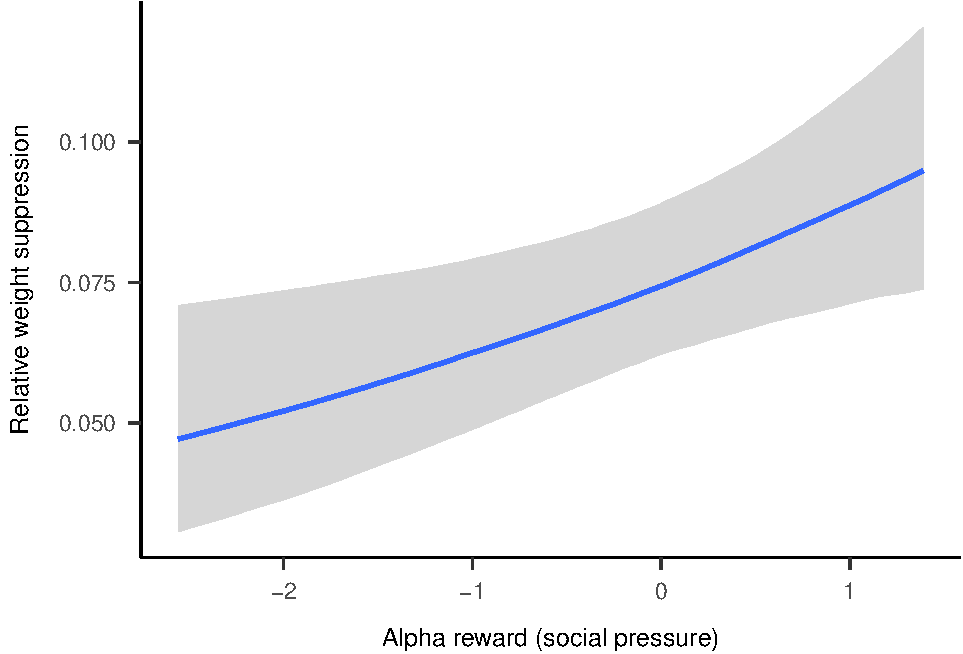
\includegraphics{046_weight_history_alpha_files/figure-latex/unnamed-chunk-10-1.pdf}

\begin{Shaded}
\begin{Highlighting}[]
\NormalTok{test\_right }\OtherTok{\textless{}{-}}\NormalTok{ bayestestR}\SpecialCharTok{::}\FunctionTok{bayesfactor\_parameters}\NormalTok{(m10, }\AttributeTok{direction =} \StringTok{"\textgreater{}"}\NormalTok{)}
\end{Highlighting}
\end{Shaded}

\begin{verbatim}
## Sampling priors, please wait...
\end{verbatim}

\begin{Shaded}
\begin{Highlighting}[]
\NormalTok{test\_right}
\end{Highlighting}
\end{Shaded}

\begin{verbatim}
## Bayes Factor (Savage-Dickey density ratio)
## 
## Parameter        |       BF
## ---------------------------
## (Intercept)      | 0.00e+00
## alpha_pos_social |     1.98
## 
## * Evidence Against The Null: 0
## *                 Direction: Right-Sided test
\end{verbatim}

\begin{Shaded}
\begin{Highlighting}[]
\FunctionTok{plot}\NormalTok{(test\_right)}
\end{Highlighting}
\end{Shaded}

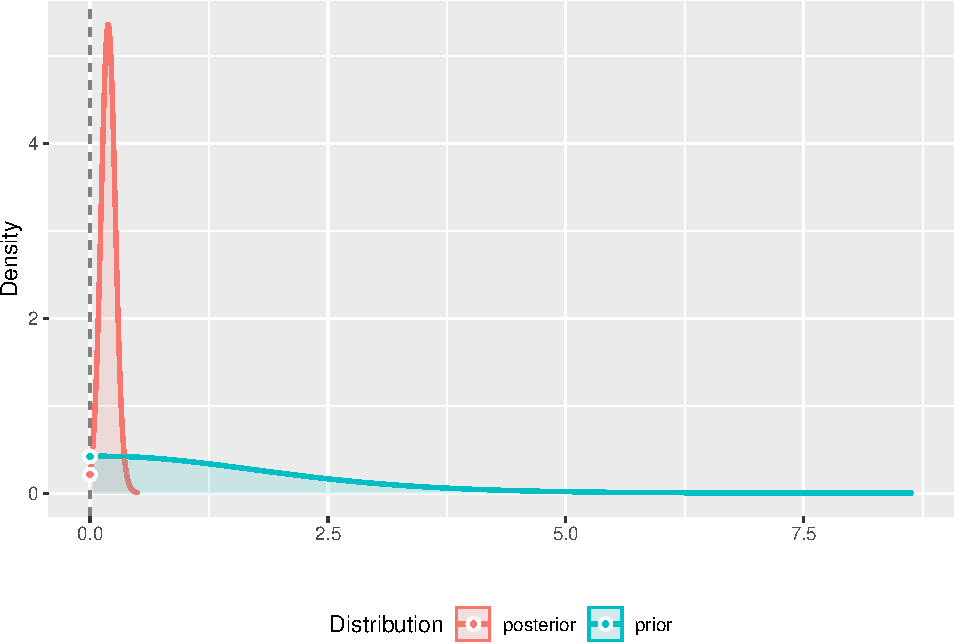
\includegraphics{046_weight_history_alpha_files/figure-latex/unnamed-chunk-10-2.pdf}

Oral control

\begin{Shaded}
\begin{Highlighting}[]
\NormalTok{m11 }\OtherTok{\textless{}{-}} \FunctionTok{brm}\NormalTok{(}
\NormalTok{  rws }\SpecialCharTok{\textasciitilde{}}\NormalTok{ oral\_control,}
  \AttributeTok{data =}\NormalTok{ foo, }
  \AttributeTok{prior =}\NormalTok{ prior\_ma,}
  \AttributeTok{family =} \FunctionTok{zero\_inflated\_beta}\NormalTok{(),}
  \AttributeTok{control =} \FunctionTok{list}\NormalTok{(}\AttributeTok{adapt\_delta =} \FloatTok{0.98}\NormalTok{),}
  \AttributeTok{iter =} \DecValTok{4000}\NormalTok{,}
  \AttributeTok{cores =} \DecValTok{6}\NormalTok{,}
  \AttributeTok{backend =} \StringTok{"cmdstan"}
\NormalTok{)}
\end{Highlighting}
\end{Shaded}

\begin{verbatim}
## Warning: Rows containing NAs were excluded from the model.
\end{verbatim}

\begin{verbatim}
## Start sampling
\end{verbatim}

\begin{verbatim}
## Running MCMC with 4 chains, at most 6 in parallel...
## 
## Chain 1 Iteration:    1 / 4000 [  0%]  (Warmup) 
## Chain 1 Iteration:  100 / 4000 [  2%]  (Warmup) 
## Chain 1 Iteration:  200 / 4000 [  5%]  (Warmup) 
## Chain 1 Iteration:  300 / 4000 [  7%]  (Warmup) 
## Chain 1 Iteration:  400 / 4000 [ 10%]  (Warmup) 
## Chain 2 Iteration:    1 / 4000 [  0%]  (Warmup) 
## Chain 2 Iteration:  100 / 4000 [  2%]  (Warmup) 
## Chain 2 Iteration:  200 / 4000 [  5%]  (Warmup) 
## Chain 2 Iteration:  300 / 4000 [  7%]  (Warmup) 
## Chain 3 Iteration:    1 / 4000 [  0%]  (Warmup) 
## Chain 3 Iteration:  100 / 4000 [  2%]  (Warmup) 
## Chain 3 Iteration:  200 / 4000 [  5%]  (Warmup) 
## Chain 3 Iteration:  300 / 4000 [  7%]  (Warmup) 
## Chain 4 Iteration:    1 / 4000 [  0%]  (Warmup) 
## Chain 4 Iteration:  100 / 4000 [  2%]  (Warmup) 
## Chain 4 Iteration:  200 / 4000 [  5%]  (Warmup) 
## Chain 1 Iteration:  500 / 4000 [ 12%]  (Warmup) 
## Chain 1 Iteration:  600 / 4000 [ 15%]  (Warmup) 
## Chain 1 Iteration:  700 / 4000 [ 17%]  (Warmup) 
## Chain 1 Iteration:  800 / 4000 [ 20%]  (Warmup) 
## Chain 2 Iteration:  400 / 4000 [ 10%]  (Warmup) 
## Chain 2 Iteration:  500 / 4000 [ 12%]  (Warmup) 
## Chain 2 Iteration:  600 / 4000 [ 15%]  (Warmup) 
## Chain 2 Iteration:  700 / 4000 [ 17%]  (Warmup) 
## Chain 3 Iteration:  400 / 4000 [ 10%]  (Warmup) 
## Chain 3 Iteration:  500 / 4000 [ 12%]  (Warmup) 
## Chain 3 Iteration:  600 / 4000 [ 15%]  (Warmup) 
## Chain 3 Iteration:  700 / 4000 [ 17%]  (Warmup) 
## Chain 4 Iteration:  300 / 4000 [  7%]  (Warmup) 
## Chain 4 Iteration:  400 / 4000 [ 10%]  (Warmup) 
## Chain 4 Iteration:  500 / 4000 [ 12%]  (Warmup) 
## Chain 1 Iteration:  900 / 4000 [ 22%]  (Warmup) 
## Chain 1 Iteration: 1000 / 4000 [ 25%]  (Warmup) 
## Chain 1 Iteration: 1100 / 4000 [ 27%]  (Warmup) 
## Chain 1 Iteration: 1200 / 4000 [ 30%]  (Warmup) 
## Chain 2 Iteration:  800 / 4000 [ 20%]  (Warmup) 
## Chain 2 Iteration:  900 / 4000 [ 22%]  (Warmup) 
## Chain 2 Iteration: 1000 / 4000 [ 25%]  (Warmup) 
## Chain 3 Iteration:  800 / 4000 [ 20%]  (Warmup) 
## Chain 3 Iteration:  900 / 4000 [ 22%]  (Warmup) 
## Chain 4 Iteration:  600 / 4000 [ 15%]  (Warmup) 
## Chain 4 Iteration:  700 / 4000 [ 17%]  (Warmup) 
## Chain 4 Iteration:  800 / 4000 [ 20%]  (Warmup) 
## Chain 1 Iteration: 1300 / 4000 [ 32%]  (Warmup) 
## Chain 1 Iteration: 1400 / 4000 [ 35%]  (Warmup) 
## Chain 1 Iteration: 1500 / 4000 [ 37%]  (Warmup) 
## Chain 2 Iteration: 1100 / 4000 [ 27%]  (Warmup) 
## Chain 2 Iteration: 1200 / 4000 [ 30%]  (Warmup) 
## Chain 2 Iteration: 1300 / 4000 [ 32%]  (Warmup) 
## Chain 3 Iteration: 1000 / 4000 [ 25%]  (Warmup) 
## Chain 3 Iteration: 1100 / 4000 [ 27%]  (Warmup) 
## Chain 3 Iteration: 1200 / 4000 [ 30%]  (Warmup) 
## Chain 3 Iteration: 1300 / 4000 [ 32%]  (Warmup) 
## Chain 4 Iteration:  900 / 4000 [ 22%]  (Warmup) 
## Chain 4 Iteration: 1000 / 4000 [ 25%]  (Warmup) 
## Chain 4 Iteration: 1100 / 4000 [ 27%]  (Warmup) 
## Chain 4 Iteration: 1200 / 4000 [ 30%]  (Warmup) 
## Chain 1 Iteration: 1600 / 4000 [ 40%]  (Warmup) 
## Chain 1 Iteration: 1700 / 4000 [ 42%]  (Warmup) 
## Chain 1 Iteration: 1800 / 4000 [ 45%]  (Warmup) 
## Chain 1 Iteration: 1900 / 4000 [ 47%]  (Warmup) 
## Chain 2 Iteration: 1400 / 4000 [ 35%]  (Warmup) 
## Chain 2 Iteration: 1500 / 4000 [ 37%]  (Warmup) 
## Chain 2 Iteration: 1600 / 4000 [ 40%]  (Warmup) 
## Chain 3 Iteration: 1400 / 4000 [ 35%]  (Warmup) 
## Chain 3 Iteration: 1500 / 4000 [ 37%]  (Warmup) 
## Chain 3 Iteration: 1600 / 4000 [ 40%]  (Warmup) 
## Chain 4 Iteration: 1300 / 4000 [ 32%]  (Warmup) 
## Chain 4 Iteration: 1400 / 4000 [ 35%]  (Warmup) 
## Chain 4 Iteration: 1500 / 4000 [ 37%]  (Warmup) 
## Chain 1 Iteration: 2000 / 4000 [ 50%]  (Warmup) 
## Chain 1 Iteration: 2001 / 4000 [ 50%]  (Sampling) 
## Chain 1 Iteration: 2100 / 4000 [ 52%]  (Sampling) 
## Chain 1 Iteration: 2200 / 4000 [ 55%]  (Sampling) 
## Chain 2 Iteration: 1700 / 4000 [ 42%]  (Warmup) 
## Chain 2 Iteration: 1800 / 4000 [ 45%]  (Warmup) 
## Chain 2 Iteration: 1900 / 4000 [ 47%]  (Warmup) 
## Chain 3 Iteration: 1700 / 4000 [ 42%]  (Warmup) 
## Chain 3 Iteration: 1800 / 4000 [ 45%]  (Warmup) 
## Chain 3 Iteration: 1900 / 4000 [ 47%]  (Warmup) 
## Chain 4 Iteration: 1600 / 4000 [ 40%]  (Warmup) 
## Chain 4 Iteration: 1700 / 4000 [ 42%]  (Warmup) 
## Chain 4 Iteration: 1800 / 4000 [ 45%]  (Warmup) 
## Chain 1 Iteration: 2300 / 4000 [ 57%]  (Sampling) 
## Chain 1 Iteration: 2400 / 4000 [ 60%]  (Sampling) 
## Chain 1 Iteration: 2500 / 4000 [ 62%]  (Sampling) 
## Chain 2 Iteration: 2000 / 4000 [ 50%]  (Warmup) 
## Chain 2 Iteration: 2001 / 4000 [ 50%]  (Sampling) 
## Chain 2 Iteration: 2100 / 4000 [ 52%]  (Sampling) 
## Chain 2 Iteration: 2200 / 4000 [ 55%]  (Sampling) 
## Chain 3 Iteration: 2000 / 4000 [ 50%]  (Warmup) 
## Chain 3 Iteration: 2001 / 4000 [ 50%]  (Sampling) 
## Chain 3 Iteration: 2100 / 4000 [ 52%]  (Sampling) 
## Chain 3 Iteration: 2200 / 4000 [ 55%]  (Sampling) 
## Chain 4 Iteration: 1900 / 4000 [ 47%]  (Warmup) 
## Chain 4 Iteration: 2000 / 4000 [ 50%]  (Warmup) 
## Chain 4 Iteration: 2001 / 4000 [ 50%]  (Sampling) 
## Chain 4 Iteration: 2100 / 4000 [ 52%]  (Sampling) 
## Chain 1 Iteration: 2600 / 4000 [ 65%]  (Sampling) 
## Chain 1 Iteration: 2700 / 4000 [ 67%]  (Sampling) 
## Chain 1 Iteration: 2800 / 4000 [ 70%]  (Sampling) 
## Chain 1 Iteration: 2900 / 4000 [ 72%]  (Sampling) 
## Chain 2 Iteration: 2300 / 4000 [ 57%]  (Sampling) 
## Chain 2 Iteration: 2400 / 4000 [ 60%]  (Sampling) 
## Chain 2 Iteration: 2500 / 4000 [ 62%]  (Sampling) 
## Chain 3 Iteration: 2300 / 4000 [ 57%]  (Sampling) 
## Chain 3 Iteration: 2400 / 4000 [ 60%]  (Sampling) 
## Chain 4 Iteration: 2200 / 4000 [ 55%]  (Sampling) 
## Chain 4 Iteration: 2300 / 4000 [ 57%]  (Sampling) 
## Chain 1 Iteration: 3000 / 4000 [ 75%]  (Sampling) 
## Chain 1 Iteration: 3100 / 4000 [ 77%]  (Sampling) 
## Chain 1 Iteration: 3200 / 4000 [ 80%]  (Sampling) 
## Chain 2 Iteration: 2600 / 4000 [ 65%]  (Sampling) 
## Chain 2 Iteration: 2700 / 4000 [ 67%]  (Sampling) 
## Chain 2 Iteration: 2800 / 4000 [ 70%]  (Sampling) 
## Chain 3 Iteration: 2500 / 4000 [ 62%]  (Sampling) 
## Chain 3 Iteration: 2600 / 4000 [ 65%]  (Sampling) 
## Chain 3 Iteration: 2700 / 4000 [ 67%]  (Sampling) 
## Chain 4 Iteration: 2400 / 4000 [ 60%]  (Sampling) 
## Chain 4 Iteration: 2500 / 4000 [ 62%]  (Sampling) 
## Chain 4 Iteration: 2600 / 4000 [ 65%]  (Sampling) 
## Chain 1 Iteration: 3300 / 4000 [ 82%]  (Sampling) 
## Chain 1 Iteration: 3400 / 4000 [ 85%]  (Sampling) 
## Chain 1 Iteration: 3500 / 4000 [ 87%]  (Sampling) 
## Chain 1 Iteration: 3600 / 4000 [ 90%]  (Sampling) 
## Chain 2 Iteration: 2900 / 4000 [ 72%]  (Sampling) 
## Chain 2 Iteration: 3000 / 4000 [ 75%]  (Sampling) 
## Chain 2 Iteration: 3100 / 4000 [ 77%]  (Sampling) 
## Chain 3 Iteration: 2800 / 4000 [ 70%]  (Sampling) 
## Chain 3 Iteration: 2900 / 4000 [ 72%]  (Sampling) 
## Chain 3 Iteration: 3000 / 4000 [ 75%]  (Sampling) 
## Chain 4 Iteration: 2700 / 4000 [ 67%]  (Sampling) 
## Chain 4 Iteration: 2800 / 4000 [ 70%]  (Sampling) 
## Chain 4 Iteration: 2900 / 4000 [ 72%]  (Sampling) 
## Chain 1 Iteration: 3700 / 4000 [ 92%]  (Sampling) 
## Chain 1 Iteration: 3800 / 4000 [ 95%]  (Sampling) 
## Chain 1 Iteration: 3900 / 4000 [ 97%]  (Sampling) 
## Chain 2 Iteration: 3200 / 4000 [ 80%]  (Sampling) 
## Chain 2 Iteration: 3300 / 4000 [ 82%]  (Sampling) 
## Chain 2 Iteration: 3400 / 4000 [ 85%]  (Sampling) 
## Chain 2 Iteration: 3500 / 4000 [ 87%]  (Sampling) 
## Chain 3 Iteration: 3100 / 4000 [ 77%]  (Sampling) 
## Chain 3 Iteration: 3200 / 4000 [ 80%]  (Sampling) 
## Chain 3 Iteration: 3300 / 4000 [ 82%]  (Sampling) 
## Chain 4 Iteration: 3000 / 4000 [ 75%]  (Sampling) 
## Chain 4 Iteration: 3100 / 4000 [ 77%]  (Sampling) 
## Chain 4 Iteration: 3200 / 4000 [ 80%]  (Sampling) 
## Chain 1 Iteration: 4000 / 4000 [100%]  (Sampling) 
## Chain 2 Iteration: 3600 / 4000 [ 90%]  (Sampling) 
## Chain 2 Iteration: 3700 / 4000 [ 92%]  (Sampling) 
## Chain 2 Iteration: 3800 / 4000 [ 95%]  (Sampling) 
## Chain 3 Iteration: 3400 / 4000 [ 85%]  (Sampling) 
## Chain 3 Iteration: 3500 / 4000 [ 87%]  (Sampling) 
## Chain 3 Iteration: 3600 / 4000 [ 90%]  (Sampling) 
## Chain 4 Iteration: 3300 / 4000 [ 82%]  (Sampling) 
## Chain 4 Iteration: 3400 / 4000 [ 85%]  (Sampling) 
## Chain 1 finished in 1.2 seconds.
## Chain 2 Iteration: 3900 / 4000 [ 97%]  (Sampling) 
## Chain 2 Iteration: 4000 / 4000 [100%]  (Sampling) 
## Chain 3 Iteration: 3700 / 4000 [ 92%]  (Sampling) 
## Chain 3 Iteration: 3800 / 4000 [ 95%]  (Sampling) 
## Chain 4 Iteration: 3500 / 4000 [ 87%]  (Sampling) 
## Chain 4 Iteration: 3600 / 4000 [ 90%]  (Sampling) 
## Chain 4 Iteration: 3700 / 4000 [ 92%]  (Sampling) 
## Chain 2 finished in 1.4 seconds.
## Chain 3 Iteration: 3900 / 4000 [ 97%]  (Sampling) 
## Chain 3 Iteration: 4000 / 4000 [100%]  (Sampling) 
## Chain 4 Iteration: 3800 / 4000 [ 95%]  (Sampling) 
## Chain 4 Iteration: 3900 / 4000 [ 97%]  (Sampling) 
## Chain 3 finished in 1.4 seconds.
## Chain 4 Iteration: 4000 / 4000 [100%]  (Sampling) 
## Chain 4 finished in 1.5 seconds.
## 
## All 4 chains finished successfully.
## Mean chain execution time: 1.4 seconds.
## Total execution time: 1.7 seconds.
\end{verbatim}

\begin{Shaded}
\begin{Highlighting}[]
\FunctionTok{summary}\NormalTok{(m11)}
\end{Highlighting}
\end{Shaded}

\begin{verbatim}
##  Family: zero_inflated_beta 
##   Links: mu = logit; phi = identity; zi = identity 
## Formula: rws ~ oral_control 
##    Data: foo (Number of observations: 101) 
## Samples: 4 chains, each with iter = 4000; warmup = 2000; thin = 1;
##          total post-warmup samples = 8000
## 
## Population-Level Effects: 
##              Estimate Est.Error l-95% CI u-95% CI Rhat Bulk_ESS Tail_ESS
## Intercept       -2.44      0.09    -2.61    -2.26 1.00     5205     4789
## oral_control     0.38      0.07     0.23     0.52 1.00     5325     4264
## 
## Family Specific Parameters: 
##     Estimate Est.Error l-95% CI u-95% CI Rhat Bulk_ESS Tail_ESS
## phi    18.15      2.75    13.14    24.03 1.00     5120     5313
## zi      0.08      0.03     0.04     0.14 1.00     6002     4688
## 
## Samples were drawn using sample(hmc). For each parameter, Bulk_ESS
## and Tail_ESS are effective sample size measures, and Rhat is the potential
## scale reduction factor on split chains (at convergence, Rhat = 1).
\end{verbatim}

\begin{Shaded}
\begin{Highlighting}[]
\NormalTok{c\_eff }\OtherTok{\textless{}{-}} \FunctionTok{conditional\_effects}\NormalTok{(m11, }\StringTok{"oral\_control"}\NormalTok{)}
\NormalTok{my\_plot }\OtherTok{\textless{}{-}} \FunctionTok{plot}\NormalTok{(c\_eff, }\AttributeTok{plot =} \ConstantTok{FALSE}\NormalTok{)[[}\DecValTok{1}\NormalTok{]] }\SpecialCharTok{+}
  \FunctionTok{labs}\NormalTok{(}
    \AttributeTok{x =} \StringTok{"Oral control"}\NormalTok{,}
    \AttributeTok{y =} \StringTok{"Relative weight suppression"}
\NormalTok{  ) }\SpecialCharTok{+}
\NormalTok{  papaja}\SpecialCharTok{::}\FunctionTok{theme\_apa}\NormalTok{()}
\NormalTok{my\_plot}
\end{Highlighting}
\end{Shaded}

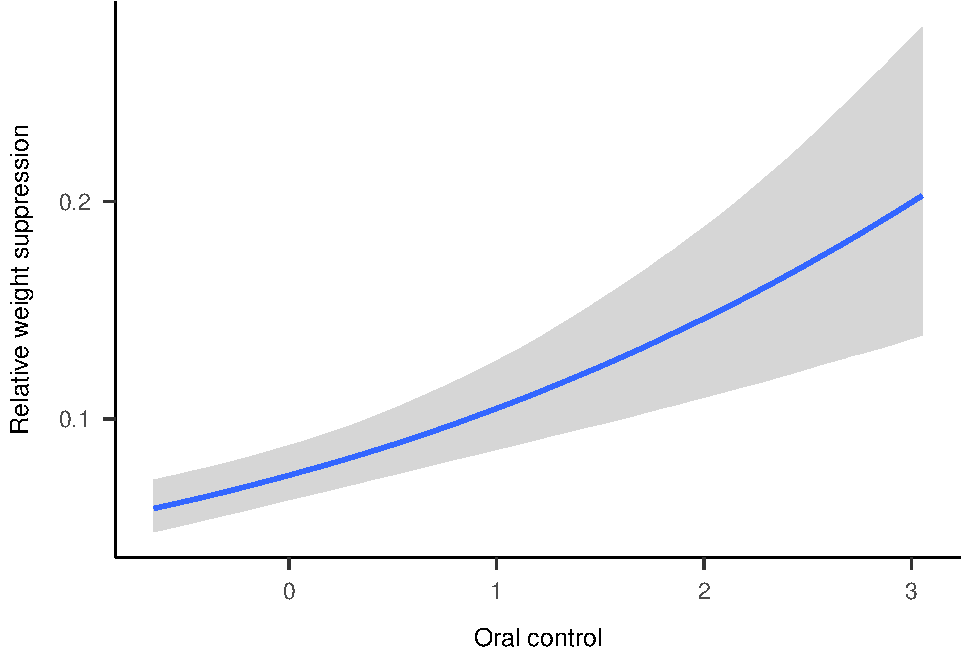
\includegraphics{046_weight_history_alpha_files/figure-latex/unnamed-chunk-11-1.pdf}

\begin{Shaded}
\begin{Highlighting}[]
\NormalTok{test\_right }\OtherTok{\textless{}{-}}\NormalTok{ bayestestR}\SpecialCharTok{::}\FunctionTok{bayesfactor\_parameters}\NormalTok{(m11, }\AttributeTok{direction =} \StringTok{"\textgreater{}"}\NormalTok{)}
\end{Highlighting}
\end{Shaded}

\begin{verbatim}
## Sampling priors, please wait...
\end{verbatim}

\begin{Shaded}
\begin{Highlighting}[]
\NormalTok{test\_right}
\end{Highlighting}
\end{Shaded}

\begin{verbatim}
## Bayes Factor (Savage-Dickey density ratio)
## 
## Parameter    |       BF
## -----------------------
## (Intercept)  | 0.00e+00
## oral_control |   420.59
## 
## * Evidence Against The Null: 0
## *                 Direction: Right-Sided test
\end{verbatim}

Dieting

\begin{Shaded}
\begin{Highlighting}[]
\NormalTok{m12 }\OtherTok{\textless{}{-}} \FunctionTok{brm}\NormalTok{(}
\NormalTok{  rws }\SpecialCharTok{\textasciitilde{}}\NormalTok{ dieting,}
  \AttributeTok{data =}\NormalTok{ foo, }
  \AttributeTok{prior =}\NormalTok{ prior\_ma,}
  \AttributeTok{family =} \FunctionTok{zero\_inflated\_beta}\NormalTok{(),}
  \AttributeTok{control =} \FunctionTok{list}\NormalTok{(}\AttributeTok{adapt\_delta =} \FloatTok{0.98}\NormalTok{),}
  \AttributeTok{iter =} \DecValTok{4000}\NormalTok{,}
  \AttributeTok{cores =} \DecValTok{6}\NormalTok{,}
  \AttributeTok{backend =} \StringTok{"cmdstan"}
\NormalTok{)}
\end{Highlighting}
\end{Shaded}

\begin{verbatim}
## Warning: Rows containing NAs were excluded from the model.
\end{verbatim}

\begin{verbatim}
## Start sampling
\end{verbatim}

\begin{verbatim}
## Running MCMC with 4 chains, at most 6 in parallel...
## 
## Chain 1 Iteration:    1 / 4000 [  0%]  (Warmup) 
## Chain 1 Iteration:  100 / 4000 [  2%]  (Warmup) 
## Chain 1 Iteration:  200 / 4000 [  5%]  (Warmup) 
## Chain 2 Iteration:    1 / 4000 [  0%]  (Warmup) 
## Chain 2 Iteration:  100 / 4000 [  2%]  (Warmup) 
## Chain 2 Iteration:  200 / 4000 [  5%]  (Warmup) 
## Chain 3 Iteration:    1 / 4000 [  0%]  (Warmup) 
## Chain 3 Iteration:  100 / 4000 [  2%]  (Warmup) 
## Chain 3 Iteration:  200 / 4000 [  5%]  (Warmup) 
## Chain 3 Iteration:  300 / 4000 [  7%]  (Warmup) 
## Chain 4 Iteration:    1 / 4000 [  0%]  (Warmup) 
## Chain 4 Iteration:  100 / 4000 [  2%]  (Warmup) 
## Chain 4 Iteration:  200 / 4000 [  5%]  (Warmup) 
## Chain 1 Iteration:  300 / 4000 [  7%]  (Warmup) 
## Chain 1 Iteration:  400 / 4000 [ 10%]  (Warmup) 
## Chain 1 Iteration:  500 / 4000 [ 12%]  (Warmup) 
## Chain 1 Iteration:  600 / 4000 [ 15%]  (Warmup) 
## Chain 2 Iteration:  300 / 4000 [  7%]  (Warmup) 
## Chain 2 Iteration:  400 / 4000 [ 10%]  (Warmup) 
## Chain 2 Iteration:  500 / 4000 [ 12%]  (Warmup) 
## Chain 2 Iteration:  600 / 4000 [ 15%]  (Warmup) 
## Chain 3 Iteration:  400 / 4000 [ 10%]  (Warmup) 
## Chain 3 Iteration:  500 / 4000 [ 12%]  (Warmup) 
## Chain 3 Iteration:  600 / 4000 [ 15%]  (Warmup) 
## Chain 4 Iteration:  300 / 4000 [  7%]  (Warmup) 
## Chain 4 Iteration:  400 / 4000 [ 10%]  (Warmup) 
## Chain 4 Iteration:  500 / 4000 [ 12%]  (Warmup) 
## Chain 4 Iteration:  600 / 4000 [ 15%]  (Warmup) 
## Chain 1 Iteration:  700 / 4000 [ 17%]  (Warmup) 
## Chain 1 Iteration:  800 / 4000 [ 20%]  (Warmup) 
## Chain 1 Iteration:  900 / 4000 [ 22%]  (Warmup) 
## Chain 2 Iteration:  700 / 4000 [ 17%]  (Warmup) 
## Chain 2 Iteration:  800 / 4000 [ 20%]  (Warmup) 
## Chain 2 Iteration:  900 / 4000 [ 22%]  (Warmup) 
## Chain 3 Iteration:  700 / 4000 [ 17%]  (Warmup) 
## Chain 3 Iteration:  800 / 4000 [ 20%]  (Warmup) 
## Chain 3 Iteration:  900 / 4000 [ 22%]  (Warmup) 
## Chain 4 Iteration:  700 / 4000 [ 17%]  (Warmup) 
## Chain 4 Iteration:  800 / 4000 [ 20%]  (Warmup) 
## Chain 4 Iteration:  900 / 4000 [ 22%]  (Warmup) 
## Chain 1 Iteration: 1000 / 4000 [ 25%]  (Warmup) 
## Chain 1 Iteration: 1100 / 4000 [ 27%]  (Warmup) 
## Chain 1 Iteration: 1200 / 4000 [ 30%]  (Warmup) 
## Chain 2 Iteration: 1000 / 4000 [ 25%]  (Warmup) 
## Chain 2 Iteration: 1100 / 4000 [ 27%]  (Warmup) 
## Chain 2 Iteration: 1200 / 4000 [ 30%]  (Warmup) 
## Chain 2 Iteration: 1300 / 4000 [ 32%]  (Warmup) 
## Chain 3 Iteration: 1000 / 4000 [ 25%]  (Warmup) 
## Chain 3 Iteration: 1100 / 4000 [ 27%]  (Warmup) 
## Chain 3 Iteration: 1200 / 4000 [ 30%]  (Warmup) 
## Chain 4 Iteration: 1000 / 4000 [ 25%]  (Warmup) 
## Chain 4 Iteration: 1100 / 4000 [ 27%]  (Warmup) 
## Chain 4 Iteration: 1200 / 4000 [ 30%]  (Warmup) 
## Chain 1 Iteration: 1300 / 4000 [ 32%]  (Warmup) 
## Chain 1 Iteration: 1400 / 4000 [ 35%]  (Warmup) 
## Chain 1 Iteration: 1500 / 4000 [ 37%]  (Warmup) 
## Chain 2 Iteration: 1400 / 4000 [ 35%]  (Warmup) 
## Chain 2 Iteration: 1500 / 4000 [ 37%]  (Warmup) 
## Chain 2 Iteration: 1600 / 4000 [ 40%]  (Warmup) 
## Chain 3 Iteration: 1300 / 4000 [ 32%]  (Warmup) 
## Chain 3 Iteration: 1400 / 4000 [ 35%]  (Warmup) 
## Chain 3 Iteration: 1500 / 4000 [ 37%]  (Warmup) 
## Chain 3 Iteration: 1600 / 4000 [ 40%]  (Warmup) 
## Chain 4 Iteration: 1300 / 4000 [ 32%]  (Warmup) 
## Chain 4 Iteration: 1400 / 4000 [ 35%]  (Warmup) 
## Chain 4 Iteration: 1500 / 4000 [ 37%]  (Warmup) 
## Chain 4 Iteration: 1600 / 4000 [ 40%]  (Warmup) 
## Chain 1 Iteration: 1600 / 4000 [ 40%]  (Warmup) 
## Chain 1 Iteration: 1700 / 4000 [ 42%]  (Warmup) 
## Chain 1 Iteration: 1800 / 4000 [ 45%]  (Warmup) 
## Chain 2 Iteration: 1700 / 4000 [ 42%]  (Warmup) 
## Chain 2 Iteration: 1800 / 4000 [ 45%]  (Warmup) 
## Chain 2 Iteration: 1900 / 4000 [ 47%]  (Warmup) 
## Chain 3 Iteration: 1700 / 4000 [ 42%]  (Warmup) 
## Chain 3 Iteration: 1800 / 4000 [ 45%]  (Warmup) 
## Chain 3 Iteration: 1900 / 4000 [ 47%]  (Warmup) 
## Chain 4 Iteration: 1700 / 4000 [ 42%]  (Warmup) 
## Chain 4 Iteration: 1800 / 4000 [ 45%]  (Warmup) 
## Chain 4 Iteration: 1900 / 4000 [ 47%]  (Warmup) 
## Chain 1 Iteration: 1900 / 4000 [ 47%]  (Warmup) 
## Chain 1 Iteration: 2000 / 4000 [ 50%]  (Warmup) 
## Chain 1 Iteration: 2001 / 4000 [ 50%]  (Sampling) 
## Chain 1 Iteration: 2100 / 4000 [ 52%]  (Sampling) 
## Chain 1 Iteration: 2200 / 4000 [ 55%]  (Sampling) 
## Chain 2 Iteration: 2000 / 4000 [ 50%]  (Warmup) 
## Chain 2 Iteration: 2001 / 4000 [ 50%]  (Sampling) 
## Chain 2 Iteration: 2100 / 4000 [ 52%]  (Sampling) 
## Chain 2 Iteration: 2200 / 4000 [ 55%]  (Sampling) 
## Chain 3 Iteration: 2000 / 4000 [ 50%]  (Warmup) 
## Chain 3 Iteration: 2001 / 4000 [ 50%]  (Sampling) 
## Chain 3 Iteration: 2100 / 4000 [ 52%]  (Sampling) 
## Chain 3 Iteration: 2200 / 4000 [ 55%]  (Sampling) 
## Chain 4 Iteration: 2000 / 4000 [ 50%]  (Warmup) 
## Chain 4 Iteration: 2001 / 4000 [ 50%]  (Sampling) 
## Chain 4 Iteration: 2100 / 4000 [ 52%]  (Sampling) 
## Chain 4 Iteration: 2200 / 4000 [ 55%]  (Sampling) 
## Chain 4 Iteration: 2300 / 4000 [ 57%]  (Sampling) 
## Chain 1 Iteration: 2300 / 4000 [ 57%]  (Sampling) 
## Chain 1 Iteration: 2400 / 4000 [ 60%]  (Sampling) 
## Chain 1 Iteration: 2500 / 4000 [ 62%]  (Sampling) 
## Chain 2 Iteration: 2300 / 4000 [ 57%]  (Sampling) 
## Chain 2 Iteration: 2400 / 4000 [ 60%]  (Sampling) 
## Chain 2 Iteration: 2500 / 4000 [ 62%]  (Sampling) 
## Chain 3 Iteration: 2300 / 4000 [ 57%]  (Sampling) 
## Chain 3 Iteration: 2400 / 4000 [ 60%]  (Sampling) 
## Chain 3 Iteration: 2500 / 4000 [ 62%]  (Sampling) 
## Chain 4 Iteration: 2400 / 4000 [ 60%]  (Sampling) 
## Chain 4 Iteration: 2500 / 4000 [ 62%]  (Sampling) 
## Chain 4 Iteration: 2600 / 4000 [ 65%]  (Sampling) 
## Chain 4 Iteration: 2700 / 4000 [ 67%]  (Sampling) 
## Chain 1 Iteration: 2600 / 4000 [ 65%]  (Sampling) 
## Chain 1 Iteration: 2700 / 4000 [ 67%]  (Sampling) 
## Chain 1 Iteration: 2800 / 4000 [ 70%]  (Sampling) 
## Chain 2 Iteration: 2600 / 4000 [ 65%]  (Sampling) 
## Chain 2 Iteration: 2700 / 4000 [ 67%]  (Sampling) 
## Chain 2 Iteration: 2800 / 4000 [ 70%]  (Sampling) 
## Chain 3 Iteration: 2600 / 4000 [ 65%]  (Sampling) 
## Chain 3 Iteration: 2700 / 4000 [ 67%]  (Sampling) 
## Chain 3 Iteration: 2800 / 4000 [ 70%]  (Sampling) 
## Chain 4 Iteration: 2800 / 4000 [ 70%]  (Sampling) 
## Chain 4 Iteration: 2900 / 4000 [ 72%]  (Sampling) 
## Chain 4 Iteration: 3000 / 4000 [ 75%]  (Sampling) 
## Chain 4 Iteration: 3100 / 4000 [ 77%]  (Sampling) 
## Chain 1 Iteration: 2900 / 4000 [ 72%]  (Sampling) 
## Chain 1 Iteration: 3000 / 4000 [ 75%]  (Sampling) 
## Chain 1 Iteration: 3100 / 4000 [ 77%]  (Sampling) 
## Chain 1 Iteration: 3200 / 4000 [ 80%]  (Sampling) 
## Chain 2 Iteration: 2900 / 4000 [ 72%]  (Sampling) 
## Chain 2 Iteration: 3000 / 4000 [ 75%]  (Sampling) 
## Chain 2 Iteration: 3100 / 4000 [ 77%]  (Sampling) 
## Chain 3 Iteration: 2900 / 4000 [ 72%]  (Sampling) 
## Chain 3 Iteration: 3000 / 4000 [ 75%]  (Sampling) 
## Chain 3 Iteration: 3100 / 4000 [ 77%]  (Sampling) 
## Chain 4 Iteration: 3200 / 4000 [ 80%]  (Sampling) 
## Chain 4 Iteration: 3300 / 4000 [ 82%]  (Sampling) 
## Chain 4 Iteration: 3400 / 4000 [ 85%]  (Sampling) 
## Chain 4 Iteration: 3500 / 4000 [ 87%]  (Sampling) 
## Chain 1 Iteration: 3300 / 4000 [ 82%]  (Sampling) 
## Chain 1 Iteration: 3400 / 4000 [ 85%]  (Sampling) 
## Chain 1 Iteration: 3500 / 4000 [ 87%]  (Sampling) 
## Chain 2 Iteration: 3200 / 4000 [ 80%]  (Sampling) 
## Chain 2 Iteration: 3300 / 4000 [ 82%]  (Sampling) 
## Chain 2 Iteration: 3400 / 4000 [ 85%]  (Sampling) 
## Chain 3 Iteration: 3200 / 4000 [ 80%]  (Sampling) 
## Chain 3 Iteration: 3300 / 4000 [ 82%]  (Sampling) 
## Chain 3 Iteration: 3400 / 4000 [ 85%]  (Sampling) 
## Chain 4 Iteration: 3600 / 4000 [ 90%]  (Sampling) 
## Chain 4 Iteration: 3700 / 4000 [ 92%]  (Sampling) 
## Chain 4 Iteration: 3800 / 4000 [ 95%]  (Sampling) 
## Chain 4 Iteration: 3900 / 4000 [ 97%]  (Sampling) 
## Chain 1 Iteration: 3600 / 4000 [ 90%]  (Sampling) 
## Chain 1 Iteration: 3700 / 4000 [ 92%]  (Sampling) 
## Chain 1 Iteration: 3800 / 4000 [ 95%]  (Sampling) 
## Chain 2 Iteration: 3500 / 4000 [ 87%]  (Sampling) 
## Chain 2 Iteration: 3600 / 4000 [ 90%]  (Sampling) 
## Chain 2 Iteration: 3700 / 4000 [ 92%]  (Sampling) 
## Chain 3 Iteration: 3500 / 4000 [ 87%]  (Sampling) 
## Chain 3 Iteration: 3600 / 4000 [ 90%]  (Sampling) 
## Chain 3 Iteration: 3700 / 4000 [ 92%]  (Sampling) 
## Chain 4 Iteration: 4000 / 4000 [100%]  (Sampling) 
## Chain 4 finished in 1.2 seconds.
## Chain 1 Iteration: 3900 / 4000 [ 97%]  (Sampling) 
## Chain 1 Iteration: 4000 / 4000 [100%]  (Sampling) 
## Chain 2 Iteration: 3800 / 4000 [ 95%]  (Sampling) 
## Chain 2 Iteration: 3900 / 4000 [ 97%]  (Sampling) 
## Chain 2 Iteration: 4000 / 4000 [100%]  (Sampling) 
## Chain 3 Iteration: 3800 / 4000 [ 95%]  (Sampling) 
## Chain 3 Iteration: 3900 / 4000 [ 97%]  (Sampling) 
## Chain 3 Iteration: 4000 / 4000 [100%]  (Sampling) 
## Chain 1 finished in 1.4 seconds.
## Chain 2 finished in 1.4 seconds.
## Chain 3 finished in 1.4 seconds.
## 
## All 4 chains finished successfully.
## Mean chain execution time: 1.3 seconds.
## Total execution time: 1.5 seconds.
\end{verbatim}

\begin{Shaded}
\begin{Highlighting}[]
\FunctionTok{summary}\NormalTok{(m12)}
\end{Highlighting}
\end{Shaded}

\begin{verbatim}
##  Family: zero_inflated_beta 
##   Links: mu = logit; phi = identity; zi = identity 
## Formula: rws ~ dieting 
##    Data: foo (Number of observations: 101) 
## Samples: 4 chains, each with iter = 4000; warmup = 2000; thin = 1;
##          total post-warmup samples = 8000
## 
## Population-Level Effects: 
##           Estimate Est.Error l-95% CI u-95% CI Rhat Bulk_ESS Tail_ESS
## Intercept    -2.45      0.09    -2.63    -2.26 1.00     4427     4234
## dieting       0.31      0.08     0.15     0.46 1.00     6188     5180
## 
## Family Specific Parameters: 
##     Estimate Est.Error l-95% CI u-95% CI Rhat Bulk_ESS Tail_ESS
## phi    16.63      2.60    11.83    22.06 1.00     4534     4566
## zi      0.08      0.03     0.03     0.14 1.00     5188     4471
## 
## Samples were drawn using sample(hmc). For each parameter, Bulk_ESS
## and Tail_ESS are effective sample size measures, and Rhat is the potential
## scale reduction factor on split chains (at convergence, Rhat = 1).
\end{verbatim}

\begin{Shaded}
\begin{Highlighting}[]
\NormalTok{c\_eff }\OtherTok{\textless{}{-}} \FunctionTok{conditional\_effects}\NormalTok{(m12, }\StringTok{"dieting"}\NormalTok{)}
\NormalTok{my\_plot }\OtherTok{\textless{}{-}} \FunctionTok{plot}\NormalTok{(c\_eff, }\AttributeTok{plot =} \ConstantTok{FALSE}\NormalTok{)[[}\DecValTok{1}\NormalTok{]] }\SpecialCharTok{+}
  \FunctionTok{labs}\NormalTok{(}
    \AttributeTok{x =} \StringTok{"Dieting"}\NormalTok{,}
    \AttributeTok{y =} \StringTok{"Relative weight suppression"}
\NormalTok{  ) }\SpecialCharTok{+}
\NormalTok{  papaja}\SpecialCharTok{::}\FunctionTok{theme\_apa}\NormalTok{()}
\NormalTok{my\_plot}
\end{Highlighting}
\end{Shaded}

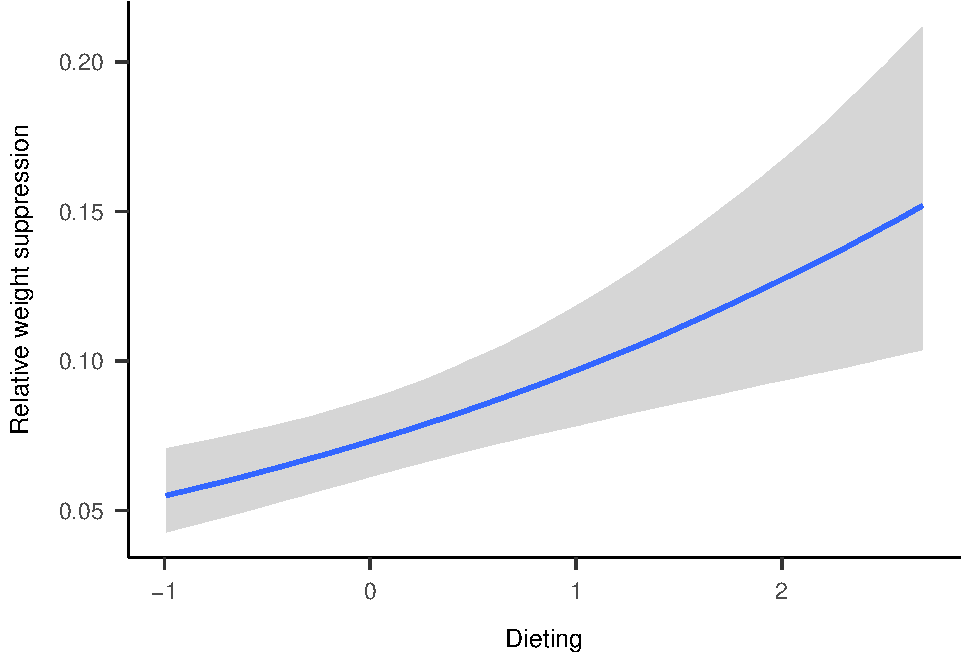
\includegraphics{046_weight_history_alpha_files/figure-latex/unnamed-chunk-12-1.pdf}

\begin{Shaded}
\begin{Highlighting}[]
\NormalTok{test\_right }\OtherTok{\textless{}{-}}\NormalTok{ bayestestR}\SpecialCharTok{::}\FunctionTok{bayesfactor\_parameters}\NormalTok{(m12, }\AttributeTok{direction =} \StringTok{"\textgreater{}"}\NormalTok{)}
\end{Highlighting}
\end{Shaded}

\begin{verbatim}
## Sampling priors, please wait...
\end{verbatim}

\begin{Shaded}
\begin{Highlighting}[]
\NormalTok{test\_right}
\end{Highlighting}
\end{Shaded}

\begin{verbatim}
## Bayes Factor (Savage-Dickey density ratio)
## 
## Parameter   |       BF
## ----------------------
## (Intercept) | 0.00e+00
## dieting     |    32.30
## 
## * Evidence Against The Null: 0
## *                 Direction: Right-Sided test
\end{verbatim}

Bulimia

\begin{Shaded}
\begin{Highlighting}[]
\NormalTok{m13 }\OtherTok{\textless{}{-}} \FunctionTok{brm}\NormalTok{(}
\NormalTok{  rws }\SpecialCharTok{\textasciitilde{}}\NormalTok{ bulimia,}
  \AttributeTok{data =}\NormalTok{ foo, }
  \AttributeTok{prior =}\NormalTok{ prior\_ma,}
  \AttributeTok{family =} \FunctionTok{zero\_inflated\_beta}\NormalTok{(),}
  \AttributeTok{control =} \FunctionTok{list}\NormalTok{(}\AttributeTok{adapt\_delta =} \FloatTok{0.98}\NormalTok{),}
  \AttributeTok{iter =} \DecValTok{4000}\NormalTok{,}
  \AttributeTok{cores =} \DecValTok{6}\NormalTok{,}
  \AttributeTok{backend =} \StringTok{"cmdstan"}
\NormalTok{)}
\end{Highlighting}
\end{Shaded}

\begin{verbatim}
## Warning: Rows containing NAs were excluded from the model.
\end{verbatim}

\begin{verbatim}
## Start sampling
\end{verbatim}

\begin{verbatim}
## Running MCMC with 4 chains, at most 6 in parallel...
## 
## Chain 1 Iteration:    1 / 4000 [  0%]  (Warmup) 
## Chain 1 Iteration:  100 / 4000 [  2%]  (Warmup) 
## Chain 1 Iteration:  200 / 4000 [  5%]  (Warmup) 
## Chain 2 Iteration:    1 / 4000 [  0%]  (Warmup) 
## Chain 2 Iteration:  100 / 4000 [  2%]  (Warmup) 
## Chain 2 Iteration:  200 / 4000 [  5%]  (Warmup) 
## Chain 2 Iteration:  300 / 4000 [  7%]  (Warmup) 
## Chain 3 Iteration:    1 / 4000 [  0%]  (Warmup) 
## Chain 3 Iteration:  100 / 4000 [  2%]  (Warmup) 
## Chain 3 Iteration:  200 / 4000 [  5%]  (Warmup) 
## Chain 4 Iteration:    1 / 4000 [  0%]  (Warmup) 
## Chain 4 Iteration:  100 / 4000 [  2%]  (Warmup) 
## Chain 4 Iteration:  200 / 4000 [  5%]  (Warmup) 
## Chain 1 Iteration:  300 / 4000 [  7%]  (Warmup) 
## Chain 1 Iteration:  400 / 4000 [ 10%]  (Warmup) 
## Chain 1 Iteration:  500 / 4000 [ 12%]  (Warmup) 
## Chain 1 Iteration:  600 / 4000 [ 15%]  (Warmup) 
## Chain 1 Iteration:  700 / 4000 [ 17%]  (Warmup) 
## Chain 2 Iteration:  400 / 4000 [ 10%]  (Warmup) 
## Chain 2 Iteration:  500 / 4000 [ 12%]  (Warmup) 
## Chain 2 Iteration:  600 / 4000 [ 15%]  (Warmup) 
## Chain 3 Iteration:  300 / 4000 [  7%]  (Warmup) 
## Chain 3 Iteration:  400 / 4000 [ 10%]  (Warmup) 
## Chain 3 Iteration:  500 / 4000 [ 12%]  (Warmup) 
## Chain 3 Iteration:  600 / 4000 [ 15%]  (Warmup) 
## Chain 4 Iteration:  300 / 4000 [  7%]  (Warmup) 
## Chain 4 Iteration:  400 / 4000 [ 10%]  (Warmup) 
## Chain 4 Iteration:  500 / 4000 [ 12%]  (Warmup) 
## Chain 4 Iteration:  600 / 4000 [ 15%]  (Warmup) 
## Chain 1 Iteration:  800 / 4000 [ 20%]  (Warmup) 
## Chain 1 Iteration:  900 / 4000 [ 22%]  (Warmup) 
## Chain 2 Iteration:  700 / 4000 [ 17%]  (Warmup) 
## Chain 2 Iteration:  800 / 4000 [ 20%]  (Warmup) 
## Chain 2 Iteration:  900 / 4000 [ 22%]  (Warmup) 
## Chain 2 Iteration: 1000 / 4000 [ 25%]  (Warmup) 
## Chain 3 Iteration:  700 / 4000 [ 17%]  (Warmup) 
## Chain 3 Iteration:  800 / 4000 [ 20%]  (Warmup) 
## Chain 3 Iteration:  900 / 4000 [ 22%]  (Warmup) 
## Chain 4 Iteration:  700 / 4000 [ 17%]  (Warmup) 
## Chain 4 Iteration:  800 / 4000 [ 20%]  (Warmup) 
## Chain 4 Iteration:  900 / 4000 [ 22%]  (Warmup) 
## Chain 1 Iteration: 1000 / 4000 [ 25%]  (Warmup) 
## Chain 1 Iteration: 1100 / 4000 [ 27%]  (Warmup) 
## Chain 1 Iteration: 1200 / 4000 [ 30%]  (Warmup) 
## Chain 1 Iteration: 1300 / 4000 [ 32%]  (Warmup) 
## Chain 2 Iteration: 1100 / 4000 [ 27%]  (Warmup) 
## Chain 2 Iteration: 1200 / 4000 [ 30%]  (Warmup) 
## Chain 2 Iteration: 1300 / 4000 [ 32%]  (Warmup) 
## Chain 3 Iteration: 1000 / 4000 [ 25%]  (Warmup) 
## Chain 3 Iteration: 1100 / 4000 [ 27%]  (Warmup) 
## Chain 3 Iteration: 1200 / 4000 [ 30%]  (Warmup) 
## Chain 4 Iteration: 1000 / 4000 [ 25%]  (Warmup) 
## Chain 4 Iteration: 1100 / 4000 [ 27%]  (Warmup) 
## Chain 4 Iteration: 1200 / 4000 [ 30%]  (Warmup) 
## Chain 1 Iteration: 1400 / 4000 [ 35%]  (Warmup) 
## Chain 1 Iteration: 1500 / 4000 [ 37%]  (Warmup) 
## Chain 1 Iteration: 1600 / 4000 [ 40%]  (Warmup) 
## Chain 2 Iteration: 1400 / 4000 [ 35%]  (Warmup) 
## Chain 2 Iteration: 1500 / 4000 [ 37%]  (Warmup) 
## Chain 2 Iteration: 1600 / 4000 [ 40%]  (Warmup) 
## Chain 3 Iteration: 1300 / 4000 [ 32%]  (Warmup) 
## Chain 3 Iteration: 1400 / 4000 [ 35%]  (Warmup) 
## Chain 3 Iteration: 1500 / 4000 [ 37%]  (Warmup) 
## Chain 3 Iteration: 1600 / 4000 [ 40%]  (Warmup) 
## Chain 4 Iteration: 1300 / 4000 [ 32%]  (Warmup) 
## Chain 4 Iteration: 1400 / 4000 [ 35%]  (Warmup) 
## Chain 4 Iteration: 1500 / 4000 [ 37%]  (Warmup) 
## Chain 4 Iteration: 1600 / 4000 [ 40%]  (Warmup) 
## Chain 1 Iteration: 1700 / 4000 [ 42%]  (Warmup) 
## Chain 1 Iteration: 1800 / 4000 [ 45%]  (Warmup) 
## Chain 1 Iteration: 1900 / 4000 [ 47%]  (Warmup) 
## Chain 2 Iteration: 1700 / 4000 [ 42%]  (Warmup) 
## Chain 2 Iteration: 1800 / 4000 [ 45%]  (Warmup) 
## Chain 2 Iteration: 1900 / 4000 [ 47%]  (Warmup) 
## Chain 3 Iteration: 1700 / 4000 [ 42%]  (Warmup) 
## Chain 3 Iteration: 1800 / 4000 [ 45%]  (Warmup) 
## Chain 3 Iteration: 1900 / 4000 [ 47%]  (Warmup) 
## Chain 4 Iteration: 1700 / 4000 [ 42%]  (Warmup) 
## Chain 4 Iteration: 1800 / 4000 [ 45%]  (Warmup) 
## Chain 4 Iteration: 1900 / 4000 [ 47%]  (Warmup) 
## Chain 1 Iteration: 2000 / 4000 [ 50%]  (Warmup) 
## Chain 1 Iteration: 2001 / 4000 [ 50%]  (Sampling) 
## Chain 1 Iteration: 2100 / 4000 [ 52%]  (Sampling) 
## Chain 1 Iteration: 2200 / 4000 [ 55%]  (Sampling) 
## Chain 2 Iteration: 2000 / 4000 [ 50%]  (Warmup) 
## Chain 2 Iteration: 2001 / 4000 [ 50%]  (Sampling) 
## Chain 2 Iteration: 2100 / 4000 [ 52%]  (Sampling) 
## Chain 2 Iteration: 2200 / 4000 [ 55%]  (Sampling) 
## Chain 3 Iteration: 2000 / 4000 [ 50%]  (Warmup) 
## Chain 3 Iteration: 2001 / 4000 [ 50%]  (Sampling) 
## Chain 3 Iteration: 2100 / 4000 [ 52%]  (Sampling) 
## Chain 3 Iteration: 2200 / 4000 [ 55%]  (Sampling) 
## Chain 4 Iteration: 2000 / 4000 [ 50%]  (Warmup) 
## Chain 4 Iteration: 2001 / 4000 [ 50%]  (Sampling) 
## Chain 4 Iteration: 2100 / 4000 [ 52%]  (Sampling) 
## Chain 4 Iteration: 2200 / 4000 [ 55%]  (Sampling) 
## Chain 1 Iteration: 2300 / 4000 [ 57%]  (Sampling) 
## Chain 1 Iteration: 2400 / 4000 [ 60%]  (Sampling) 
## Chain 1 Iteration: 2500 / 4000 [ 62%]  (Sampling) 
## Chain 2 Iteration: 2300 / 4000 [ 57%]  (Sampling) 
## Chain 2 Iteration: 2400 / 4000 [ 60%]  (Sampling) 
## Chain 2 Iteration: 2500 / 4000 [ 62%]  (Sampling) 
## Chain 3 Iteration: 2300 / 4000 [ 57%]  (Sampling) 
## Chain 3 Iteration: 2400 / 4000 [ 60%]  (Sampling) 
## Chain 3 Iteration: 2500 / 4000 [ 62%]  (Sampling) 
## Chain 3 Iteration: 2600 / 4000 [ 65%]  (Sampling) 
## Chain 4 Iteration: 2300 / 4000 [ 57%]  (Sampling) 
## Chain 4 Iteration: 2400 / 4000 [ 60%]  (Sampling) 
## Chain 4 Iteration: 2500 / 4000 [ 62%]  (Sampling) 
## Chain 4 Iteration: 2600 / 4000 [ 65%]  (Sampling) 
## Chain 1 Iteration: 2600 / 4000 [ 65%]  (Sampling) 
## Chain 1 Iteration: 2700 / 4000 [ 67%]  (Sampling) 
## Chain 1 Iteration: 2800 / 4000 [ 70%]  (Sampling) 
## Chain 2 Iteration: 2600 / 4000 [ 65%]  (Sampling) 
## Chain 2 Iteration: 2700 / 4000 [ 67%]  (Sampling) 
## Chain 2 Iteration: 2800 / 4000 [ 70%]  (Sampling) 
## Chain 2 Iteration: 2900 / 4000 [ 72%]  (Sampling) 
## Chain 3 Iteration: 2700 / 4000 [ 67%]  (Sampling) 
## Chain 3 Iteration: 2800 / 4000 [ 70%]  (Sampling) 
## Chain 3 Iteration: 2900 / 4000 [ 72%]  (Sampling) 
## Chain 4 Iteration: 2700 / 4000 [ 67%]  (Sampling) 
## Chain 4 Iteration: 2800 / 4000 [ 70%]  (Sampling) 
## Chain 4 Iteration: 2900 / 4000 [ 72%]  (Sampling) 
## Chain 1 Iteration: 2900 / 4000 [ 72%]  (Sampling) 
## Chain 1 Iteration: 3000 / 4000 [ 75%]  (Sampling) 
## Chain 1 Iteration: 3100 / 4000 [ 77%]  (Sampling) 
## Chain 2 Iteration: 3000 / 4000 [ 75%]  (Sampling) 
## Chain 2 Iteration: 3100 / 4000 [ 77%]  (Sampling) 
## Chain 2 Iteration: 3200 / 4000 [ 80%]  (Sampling) 
## Chain 3 Iteration: 3000 / 4000 [ 75%]  (Sampling) 
## Chain 3 Iteration: 3100 / 4000 [ 77%]  (Sampling) 
## Chain 3 Iteration: 3200 / 4000 [ 80%]  (Sampling) 
## Chain 4 Iteration: 3000 / 4000 [ 75%]  (Sampling) 
## Chain 4 Iteration: 3100 / 4000 [ 77%]  (Sampling) 
## Chain 4 Iteration: 3200 / 4000 [ 80%]  (Sampling) 
## Chain 4 Iteration: 3300 / 4000 [ 82%]  (Sampling) 
## Chain 1 Iteration: 3200 / 4000 [ 80%]  (Sampling) 
## Chain 1 Iteration: 3300 / 4000 [ 82%]  (Sampling) 
## Chain 2 Iteration: 3300 / 4000 [ 82%]  (Sampling) 
## Chain 2 Iteration: 3400 / 4000 [ 85%]  (Sampling) 
## Chain 2 Iteration: 3500 / 4000 [ 87%]  (Sampling) 
## Chain 3 Iteration: 3300 / 4000 [ 82%]  (Sampling) 
## Chain 3 Iteration: 3400 / 4000 [ 85%]  (Sampling) 
## Chain 3 Iteration: 3500 / 4000 [ 87%]  (Sampling) 
## Chain 3 Iteration: 3600 / 4000 [ 90%]  (Sampling) 
## Chain 4 Iteration: 3400 / 4000 [ 85%]  (Sampling) 
## Chain 4 Iteration: 3500 / 4000 [ 87%]  (Sampling) 
## Chain 4 Iteration: 3600 / 4000 [ 90%]  (Sampling) 
## Chain 1 Iteration: 3400 / 4000 [ 85%]  (Sampling) 
## Chain 1 Iteration: 3500 / 4000 [ 87%]  (Sampling) 
## Chain 1 Iteration: 3600 / 4000 [ 90%]  (Sampling) 
## Chain 2 Iteration: 3600 / 4000 [ 90%]  (Sampling) 
## Chain 2 Iteration: 3700 / 4000 [ 92%]  (Sampling) 
## Chain 2 Iteration: 3800 / 4000 [ 95%]  (Sampling) 
## Chain 3 Iteration: 3700 / 4000 [ 92%]  (Sampling) 
## Chain 3 Iteration: 3800 / 4000 [ 95%]  (Sampling) 
## Chain 3 Iteration: 3900 / 4000 [ 97%]  (Sampling) 
## Chain 4 Iteration: 3700 / 4000 [ 92%]  (Sampling) 
## Chain 4 Iteration: 3800 / 4000 [ 95%]  (Sampling) 
## Chain 4 Iteration: 3900 / 4000 [ 97%]  (Sampling) 
## Chain 4 Iteration: 4000 / 4000 [100%]  (Sampling) 
## Chain 4 finished in 1.3 seconds.
## Chain 1 Iteration: 3700 / 4000 [ 92%]  (Sampling) 
## Chain 1 Iteration: 3800 / 4000 [ 95%]  (Sampling) 
## Chain 1 Iteration: 3900 / 4000 [ 97%]  (Sampling) 
## Chain 2 Iteration: 3900 / 4000 [ 97%]  (Sampling) 
## Chain 2 Iteration: 4000 / 4000 [100%]  (Sampling) 
## Chain 3 Iteration: 4000 / 4000 [100%]  (Sampling) 
## Chain 2 finished in 1.4 seconds.
## Chain 3 finished in 1.3 seconds.
## Chain 1 Iteration: 4000 / 4000 [100%]  (Sampling) 
## Chain 1 finished in 1.5 seconds.
## 
## All 4 chains finished successfully.
## Mean chain execution time: 1.4 seconds.
## Total execution time: 1.6 seconds.
\end{verbatim}

\begin{Shaded}
\begin{Highlighting}[]
\FunctionTok{summary}\NormalTok{(m13)}
\end{Highlighting}
\end{Shaded}

\begin{verbatim}
##  Family: zero_inflated_beta 
##   Links: mu = logit; phi = identity; zi = identity 
## Formula: rws ~ bulimia 
##    Data: foo (Number of observations: 101) 
## Samples: 4 chains, each with iter = 4000; warmup = 2000; thin = 1;
##          total post-warmup samples = 8000
## 
## Population-Level Effects: 
##           Estimate Est.Error l-95% CI u-95% CI Rhat Bulk_ESS Tail_ESS
## Intercept    -2.45      0.09    -2.63    -2.26 1.00     4979     5397
## bulimia       0.29      0.08     0.13     0.45 1.00     5300     5129
## 
## Family Specific Parameters: 
##     Estimate Est.Error l-95% CI u-95% CI Rhat Bulk_ESS Tail_ESS
## phi    16.33      2.52    11.63    21.62 1.00     4542     5058
## zi      0.08      0.03     0.03     0.14 1.00     5655     4430
## 
## Samples were drawn using sample(hmc). For each parameter, Bulk_ESS
## and Tail_ESS are effective sample size measures, and Rhat is the potential
## scale reduction factor on split chains (at convergence, Rhat = 1).
\end{verbatim}

\begin{Shaded}
\begin{Highlighting}[]
\NormalTok{c\_eff }\OtherTok{\textless{}{-}} \FunctionTok{conditional\_effects}\NormalTok{(m13, }\StringTok{"bulimia"}\NormalTok{)}
\NormalTok{my\_plot }\OtherTok{\textless{}{-}} \FunctionTok{plot}\NormalTok{(c\_eff, }\AttributeTok{plot =} \ConstantTok{FALSE}\NormalTok{)[[}\DecValTok{1}\NormalTok{]] }\SpecialCharTok{+}
  \FunctionTok{labs}\NormalTok{(}
    \AttributeTok{x =} \StringTok{"Bulimia"}\NormalTok{,}
    \AttributeTok{y =} \StringTok{"Relative weight suppression"}
\NormalTok{  ) }\SpecialCharTok{+}
\NormalTok{  papaja}\SpecialCharTok{::}\FunctionTok{theme\_apa}\NormalTok{()}
\NormalTok{my\_plot}
\end{Highlighting}
\end{Shaded}

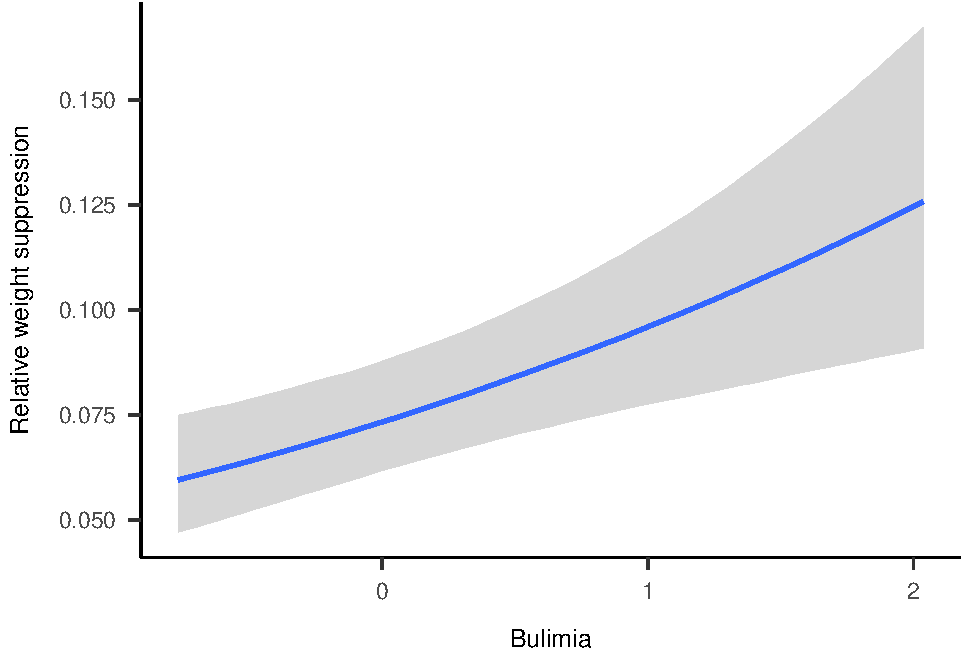
\includegraphics{046_weight_history_alpha_files/figure-latex/unnamed-chunk-13-1.pdf}

\begin{Shaded}
\begin{Highlighting}[]
\NormalTok{test\_right }\OtherTok{\textless{}{-}}\NormalTok{ bayestestR}\SpecialCharTok{::}\FunctionTok{bayesfactor\_parameters}\NormalTok{(m13, }\AttributeTok{direction =} \StringTok{"\textgreater{}"}\NormalTok{)}
\end{Highlighting}
\end{Shaded}

\begin{verbatim}
## Sampling priors, please wait...
\end{verbatim}

\begin{Shaded}
\begin{Highlighting}[]
\NormalTok{test\_right}
\end{Highlighting}
\end{Shaded}

\begin{verbatim}
## Bayes Factor (Savage-Dickey density ratio)
## 
## Parameter   |       BF
## ----------------------
## (Intercept) | 0.00e+00
## bulimia     |    13.23
## 
## * Evidence Against The Null: 0
## *                 Direction: Right-Sided test
\end{verbatim}

Difference between the present weight and the predicted weight that the
participant expect, if she/he does not try to control her/his eating
behavior

\begin{Shaded}
\begin{Highlighting}[]
\NormalTok{foo}\SpecialCharTok{$}\NormalTok{predicted\_weight }\OtherTok{\textless{}{-}} \FunctionTok{recode\_predicted\_weight}\NormalTok{(foo)}

\NormalTok{imp }\OtherTok{\textless{}{-}}\NormalTok{ mice}\SpecialCharTok{::}\FunctionTok{mice}\NormalTok{(foo, }\AttributeTok{method =} \StringTok{"mean"}\NormalTok{, }\AttributeTok{m =} \DecValTok{1}\NormalTok{) }\CommentTok{\# Impute data}
\end{Highlighting}
\end{Shaded}

\begin{verbatim}
## 
##  iter imp variable
##   1   1  v_food  v_social  t_food  t_social  z_food  z_social  alpha_neg_food  alpha_neg_social  alpha_pos_food  alpha_pos_social  bsq14_tot  ros_tot  dass21_stress  dass21_anxiety  dass21_dep  sias  mps_ps  mps_o  mps_cmd  mps_pepc  orto_tot  dieting  bulimia  oral_control  eat26_at_risk  eat26  age  present_weight  height  highest_weight  predicted_weight  ws  rws  BMI
##   2   1  v_food  v_social  t_food  t_social  z_food  z_social  alpha_neg_food  alpha_neg_social  alpha_pos_food  alpha_pos_social  bsq14_tot  ros_tot  dass21_stress  dass21_anxiety  dass21_dep  sias  mps_ps  mps_o  mps_cmd  mps_pepc  orto_tot  dieting  bulimia  oral_control  eat26_at_risk  eat26  age  present_weight  height  highest_weight  predicted_weight  ws  rws  BMI
##   3   1  v_food  v_social  t_food  t_social  z_food  z_social  alpha_neg_food  alpha_neg_social  alpha_pos_food  alpha_pos_social  bsq14_tot  ros_tot  dass21_stress  dass21_anxiety  dass21_dep  sias  mps_ps  mps_o  mps_cmd  mps_pepc  orto_tot  dieting  bulimia  oral_control  eat26_at_risk  eat26  age  present_weight  height  highest_weight  predicted_weight  ws  rws  BMI
##   4   1  v_food  v_social  t_food  t_social  z_food  z_social  alpha_neg_food  alpha_neg_social  alpha_pos_food  alpha_pos_social  bsq14_tot  ros_tot  dass21_stress  dass21_anxiety  dass21_dep  sias  mps_ps  mps_o  mps_cmd  mps_pepc  orto_tot  dieting  bulimia  oral_control  eat26_at_risk  eat26  age  present_weight  height  highest_weight  predicted_weight  ws  rws  BMI
##   5   1  v_food  v_social  t_food  t_social  z_food  z_social  alpha_neg_food  alpha_neg_social  alpha_pos_food  alpha_pos_social  bsq14_tot  ros_tot  dass21_stress  dass21_anxiety  dass21_dep  sias  mps_ps  mps_o  mps_cmd  mps_pepc  orto_tot  dieting  bulimia  oral_control  eat26_at_risk  eat26  age  present_weight  height  highest_weight  predicted_weight  ws  rws  BMI
\end{verbatim}

\begin{verbatim}
## Warning: Number of logged events: 191
\end{verbatim}

\begin{Shaded}
\begin{Highlighting}[]
\NormalTok{data\_imp }\OtherTok{\textless{}{-}} \FunctionTok{complete}\NormalTok{(imp) }\CommentTok{\# Store data}
\end{Highlighting}
\end{Shaded}

Difference between predicted weight and actual weight

\begin{Shaded}
\begin{Highlighting}[]
\NormalTok{data\_imp}\SpecialCharTok{$}\NormalTok{pred\_weight\_dif }\OtherTok{\textless{}{-}}\NormalTok{ data\_imp}\SpecialCharTok{$}\NormalTok{predicted\_weight }\SpecialCharTok{{-}}\NormalTok{ data\_imp}\SpecialCharTok{$}\NormalTok{present\_weight}

\NormalTok{data\_imp }\SpecialCharTok{\%\textgreater{}\%} 
  \FunctionTok{group\_by}\NormalTok{(Group) }\SpecialCharTok{\%\textgreater{}\%} 
  \FunctionTok{summarise}\NormalTok{(}
    \AttributeTok{avg\_dif =} \FunctionTok{mean}\NormalTok{(pred\_weight\_dif, }\AttributeTok{trim =} \FloatTok{0.1}\NormalTok{)}
\NormalTok{  )}
\end{Highlighting}
\end{Shaded}

\begin{verbatim}
## # A tibble: 3 x 2
##   Group   avg_dif
##   <fct>     <dbl>
## 1 at risk    4.25
## 2 control    1.74
## 3 patient    3.43
\end{verbatim}

\begin{Shaded}
\begin{Highlighting}[]
\FunctionTok{hist}\NormalTok{(data\_imp}\SpecialCharTok{$}\NormalTok{pred\_weight\_dif)}
\end{Highlighting}
\end{Shaded}

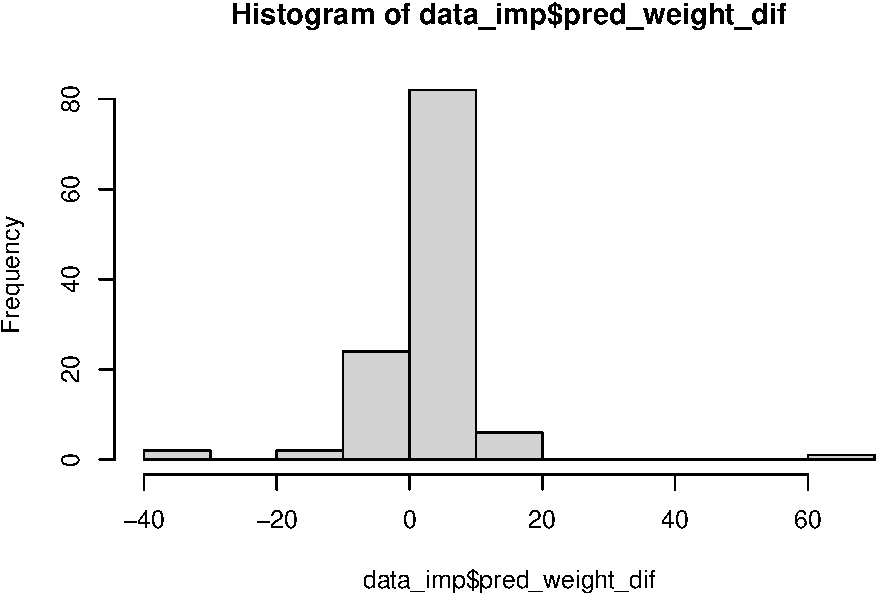
\includegraphics{046_weight_history_alpha_files/figure-latex/unnamed-chunk-15-1.pdf}

\begin{Shaded}
\begin{Highlighting}[]
\CommentTok{\# Control as baseline group}
\NormalTok{data\_imp}\SpecialCharTok{$}\NormalTok{Group }\OtherTok{\textless{}{-}} \FunctionTok{relevel}\NormalTok{(data\_imp}\SpecialCharTok{$}\NormalTok{Group, }\AttributeTok{ref =} \StringTok{"control"}\NormalTok{)}
\end{Highlighting}
\end{Shaded}

Predicted weight difference

\begin{Shaded}
\begin{Highlighting}[]
\NormalTok{m14 }\OtherTok{\textless{}{-}} \FunctionTok{brm}\NormalTok{(}
\NormalTok{  pred\_weight\_dif }\SpecialCharTok{\textasciitilde{}}\NormalTok{ Group,}
  \AttributeTok{data =}\NormalTok{ data\_imp, }
  \AttributeTok{prior =}\NormalTok{ prior\_ma,}
  \AttributeTok{family =} \FunctionTok{student}\NormalTok{(),}
  \AttributeTok{control =} \FunctionTok{list}\NormalTok{(}\AttributeTok{adapt\_delta =} \FloatTok{0.98}\NormalTok{),}
  \AttributeTok{iter =} \DecValTok{4000}\NormalTok{,}
  \AttributeTok{cores =} \DecValTok{6}\NormalTok{,}
  \AttributeTok{backend =} \StringTok{"cmdstan"}
\NormalTok{)}
\end{Highlighting}
\end{Shaded}

\begin{verbatim}
## Start sampling
\end{verbatim}

\begin{verbatim}
## Running MCMC with 4 chains, at most 6 in parallel...
## 
## Chain 1 Iteration:    1 / 4000 [  0%]  (Warmup) 
## Chain 1 Iteration:  100 / 4000 [  2%]  (Warmup) 
## Chain 2 Iteration:    1 / 4000 [  0%]  (Warmup) 
## Chain 2 Iteration:  100 / 4000 [  2%]  (Warmup) 
## Chain 2 Iteration:  200 / 4000 [  5%]  (Warmup) 
## Chain 3 Iteration:    1 / 4000 [  0%]  (Warmup) 
## Chain 3 Iteration:  100 / 4000 [  2%]  (Warmup) 
## Chain 3 Iteration:  200 / 4000 [  5%]  (Warmup) 
## Chain 3 Iteration:  300 / 4000 [  7%]  (Warmup) 
## Chain 3 Iteration:  400 / 4000 [ 10%]  (Warmup) 
## Chain 3 Iteration:  500 / 4000 [ 12%]  (Warmup) 
## Chain 3 Iteration:  600 / 4000 [ 15%]  (Warmup) 
## Chain 4 Iteration:    1 / 4000 [  0%]  (Warmup) 
## Chain 4 Iteration:  100 / 4000 [  2%]  (Warmup) 
## Chain 4 Iteration:  200 / 4000 [  5%]  (Warmup) 
## Chain 4 Iteration:  300 / 4000 [  7%]  (Warmup) 
## Chain 4 Iteration:  400 / 4000 [ 10%]  (Warmup) 
## Chain 4 Iteration:  500 / 4000 [ 12%]  (Warmup) 
## Chain 4 Iteration:  600 / 4000 [ 15%]  (Warmup) 
## Chain 4 Iteration:  700 / 4000 [ 17%]  (Warmup) 
## Chain 1 Iteration:  200 / 4000 [  5%]  (Warmup) 
## Chain 1 Iteration:  300 / 4000 [  7%]  (Warmup) 
## Chain 1 Iteration:  400 / 4000 [ 10%]  (Warmup) 
## Chain 1 Iteration:  500 / 4000 [ 12%]  (Warmup) 
## Chain 1 Iteration:  600 / 4000 [ 15%]  (Warmup) 
## Chain 1 Iteration:  700 / 4000 [ 17%]  (Warmup) 
## Chain 1 Iteration:  800 / 4000 [ 20%]  (Warmup) 
## Chain 1 Iteration:  900 / 4000 [ 22%]  (Warmup) 
## Chain 1 Iteration: 1000 / 4000 [ 25%]  (Warmup) 
## Chain 1 Iteration: 1100 / 4000 [ 27%]  (Warmup) 
## Chain 1 Iteration: 1200 / 4000 [ 30%]  (Warmup) 
## Chain 1 Iteration: 1300 / 4000 [ 32%]  (Warmup) 
## Chain 1 Iteration: 1400 / 4000 [ 35%]  (Warmup) 
## Chain 1 Iteration: 1500 / 4000 [ 37%]  (Warmup) 
## Chain 1 Iteration: 1600 / 4000 [ 40%]  (Warmup) 
## Chain 1 Iteration: 1700 / 4000 [ 42%]  (Warmup) 
## Chain 1 Iteration: 1800 / 4000 [ 45%]  (Warmup) 
## Chain 1 Iteration: 1900 / 4000 [ 47%]  (Warmup) 
## Chain 2 Iteration:  300 / 4000 [  7%]  (Warmup) 
## Chain 2 Iteration:  400 / 4000 [ 10%]  (Warmup) 
## Chain 2 Iteration:  500 / 4000 [ 12%]  (Warmup) 
## Chain 2 Iteration:  600 / 4000 [ 15%]  (Warmup) 
## Chain 2 Iteration:  700 / 4000 [ 17%]  (Warmup) 
## Chain 2 Iteration:  800 / 4000 [ 20%]  (Warmup) 
## Chain 2 Iteration:  900 / 4000 [ 22%]  (Warmup) 
## Chain 2 Iteration: 1000 / 4000 [ 25%]  (Warmup) 
## Chain 2 Iteration: 1100 / 4000 [ 27%]  (Warmup) 
## Chain 2 Iteration: 1200 / 4000 [ 30%]  (Warmup) 
## Chain 2 Iteration: 1300 / 4000 [ 32%]  (Warmup) 
## Chain 2 Iteration: 1400 / 4000 [ 35%]  (Warmup) 
## Chain 2 Iteration: 1500 / 4000 [ 37%]  (Warmup) 
## Chain 2 Iteration: 1600 / 4000 [ 40%]  (Warmup) 
## Chain 2 Iteration: 1700 / 4000 [ 42%]  (Warmup) 
## Chain 2 Iteration: 1800 / 4000 [ 45%]  (Warmup) 
## Chain 2 Iteration: 1900 / 4000 [ 47%]  (Warmup) 
## Chain 2 Iteration: 2000 / 4000 [ 50%]  (Warmup) 
## Chain 3 Iteration:  700 / 4000 [ 17%]  (Warmup) 
## Chain 3 Iteration:  800 / 4000 [ 20%]  (Warmup) 
## Chain 3 Iteration:  900 / 4000 [ 22%]  (Warmup) 
## Chain 3 Iteration: 1000 / 4000 [ 25%]  (Warmup) 
## Chain 3 Iteration: 1100 / 4000 [ 27%]  (Warmup) 
## Chain 3 Iteration: 1200 / 4000 [ 30%]  (Warmup) 
## Chain 3 Iteration: 1300 / 4000 [ 32%]  (Warmup) 
## Chain 3 Iteration: 1400 / 4000 [ 35%]  (Warmup) 
## Chain 3 Iteration: 1500 / 4000 [ 37%]  (Warmup) 
## Chain 3 Iteration: 1600 / 4000 [ 40%]  (Warmup) 
## Chain 3 Iteration: 1700 / 4000 [ 42%]  (Warmup) 
## Chain 3 Iteration: 1800 / 4000 [ 45%]  (Warmup) 
## Chain 3 Iteration: 1900 / 4000 [ 47%]  (Warmup) 
## Chain 3 Iteration: 2000 / 4000 [ 50%]  (Warmup) 
## Chain 4 Iteration:  800 / 4000 [ 20%]  (Warmup) 
## Chain 4 Iteration:  900 / 4000 [ 22%]  (Warmup) 
## Chain 4 Iteration: 1000 / 4000 [ 25%]  (Warmup) 
## Chain 4 Iteration: 1100 / 4000 [ 27%]  (Warmup) 
## Chain 4 Iteration: 1200 / 4000 [ 30%]  (Warmup) 
## Chain 4 Iteration: 1300 / 4000 [ 32%]  (Warmup) 
## Chain 4 Iteration: 1400 / 4000 [ 35%]  (Warmup) 
## Chain 4 Iteration: 1500 / 4000 [ 37%]  (Warmup) 
## Chain 4 Iteration: 1600 / 4000 [ 40%]  (Warmup) 
## Chain 4 Iteration: 1700 / 4000 [ 42%]  (Warmup) 
## Chain 4 Iteration: 1800 / 4000 [ 45%]  (Warmup) 
## Chain 4 Iteration: 1900 / 4000 [ 47%]  (Warmup) 
## Chain 4 Iteration: 2000 / 4000 [ 50%]  (Warmup) 
## Chain 4 Iteration: 2001 / 4000 [ 50%]  (Sampling) 
## Chain 1 Iteration: 2000 / 4000 [ 50%]  (Warmup) 
## Chain 1 Iteration: 2001 / 4000 [ 50%]  (Sampling) 
## Chain 1 Iteration: 2100 / 4000 [ 52%]  (Sampling) 
## Chain 1 Iteration: 2200 / 4000 [ 55%]  (Sampling) 
## Chain 1 Iteration: 2300 / 4000 [ 57%]  (Sampling) 
## Chain 1 Iteration: 2400 / 4000 [ 60%]  (Sampling) 
## Chain 1 Iteration: 2500 / 4000 [ 62%]  (Sampling) 
## Chain 2 Iteration: 2001 / 4000 [ 50%]  (Sampling) 
## Chain 2 Iteration: 2100 / 4000 [ 52%]  (Sampling) 
## Chain 2 Iteration: 2200 / 4000 [ 55%]  (Sampling) 
## Chain 2 Iteration: 2300 / 4000 [ 57%]  (Sampling) 
## Chain 2 Iteration: 2400 / 4000 [ 60%]  (Sampling) 
## Chain 2 Iteration: 2500 / 4000 [ 62%]  (Sampling) 
## Chain 2 Iteration: 2600 / 4000 [ 65%]  (Sampling) 
## Chain 2 Iteration: 2700 / 4000 [ 67%]  (Sampling) 
## Chain 2 Iteration: 2800 / 4000 [ 70%]  (Sampling) 
## Chain 2 Iteration: 2900 / 4000 [ 72%]  (Sampling) 
## Chain 3 Iteration: 2001 / 4000 [ 50%]  (Sampling) 
## Chain 3 Iteration: 2100 / 4000 [ 52%]  (Sampling) 
## Chain 3 Iteration: 2200 / 4000 [ 55%]  (Sampling) 
## Chain 3 Iteration: 2300 / 4000 [ 57%]  (Sampling) 
## Chain 3 Iteration: 2400 / 4000 [ 60%]  (Sampling) 
## Chain 3 Iteration: 2500 / 4000 [ 62%]  (Sampling) 
## Chain 3 Iteration: 2600 / 4000 [ 65%]  (Sampling) 
## Chain 3 Iteration: 2700 / 4000 [ 67%]  (Sampling) 
## Chain 3 Iteration: 2800 / 4000 [ 70%]  (Sampling) 
## Chain 3 Iteration: 2900 / 4000 [ 72%]  (Sampling) 
## Chain 3 Iteration: 3000 / 4000 [ 75%]  (Sampling) 
## Chain 3 Iteration: 3100 / 4000 [ 77%]  (Sampling) 
## Chain 4 Iteration: 2100 / 4000 [ 52%]  (Sampling) 
## Chain 4 Iteration: 2200 / 4000 [ 55%]  (Sampling) 
## Chain 4 Iteration: 2300 / 4000 [ 57%]  (Sampling) 
## Chain 4 Iteration: 2400 / 4000 [ 60%]  (Sampling) 
## Chain 4 Iteration: 2500 / 4000 [ 62%]  (Sampling) 
## Chain 4 Iteration: 2600 / 4000 [ 65%]  (Sampling) 
## Chain 4 Iteration: 2700 / 4000 [ 67%]  (Sampling) 
## Chain 4 Iteration: 2800 / 4000 [ 70%]  (Sampling) 
## Chain 4 Iteration: 2900 / 4000 [ 72%]  (Sampling) 
## Chain 4 Iteration: 3000 / 4000 [ 75%]  (Sampling) 
## Chain 1 Iteration: 2600 / 4000 [ 65%]  (Sampling) 
## Chain 1 Iteration: 2700 / 4000 [ 67%]  (Sampling) 
## Chain 1 Iteration: 2800 / 4000 [ 70%]  (Sampling) 
## Chain 1 Iteration: 2900 / 4000 [ 72%]  (Sampling) 
## Chain 1 Iteration: 3000 / 4000 [ 75%]  (Sampling) 
## Chain 2 Iteration: 3000 / 4000 [ 75%]  (Sampling) 
## Chain 2 Iteration: 3100 / 4000 [ 77%]  (Sampling) 
## Chain 2 Iteration: 3200 / 4000 [ 80%]  (Sampling) 
## Chain 2 Iteration: 3300 / 4000 [ 82%]  (Sampling) 
## Chain 2 Iteration: 3400 / 4000 [ 85%]  (Sampling) 
## Chain 2 Iteration: 3500 / 4000 [ 87%]  (Sampling) 
## Chain 2 Iteration: 3600 / 4000 [ 90%]  (Sampling) 
## Chain 2 Iteration: 3700 / 4000 [ 92%]  (Sampling) 
## Chain 2 Iteration: 3800 / 4000 [ 95%]  (Sampling) 
## Chain 2 Iteration: 3900 / 4000 [ 97%]  (Sampling) 
## Chain 2 Iteration: 4000 / 4000 [100%]  (Sampling) 
## Chain 3 Iteration: 3200 / 4000 [ 80%]  (Sampling) 
## Chain 3 Iteration: 3300 / 4000 [ 82%]  (Sampling) 
## Chain 3 Iteration: 3400 / 4000 [ 85%]  (Sampling) 
## Chain 3 Iteration: 3500 / 4000 [ 87%]  (Sampling) 
## Chain 3 Iteration: 3600 / 4000 [ 90%]  (Sampling) 
## Chain 3 Iteration: 3700 / 4000 [ 92%]  (Sampling) 
## Chain 3 Iteration: 3800 / 4000 [ 95%]  (Sampling) 
## Chain 3 Iteration: 3900 / 4000 [ 97%]  (Sampling) 
## Chain 3 Iteration: 4000 / 4000 [100%]  (Sampling) 
## Chain 4 Iteration: 3100 / 4000 [ 77%]  (Sampling) 
## Chain 4 Iteration: 3200 / 4000 [ 80%]  (Sampling) 
## Chain 4 Iteration: 3300 / 4000 [ 82%]  (Sampling) 
## Chain 4 Iteration: 3400 / 4000 [ 85%]  (Sampling) 
## Chain 4 Iteration: 3500 / 4000 [ 87%]  (Sampling) 
## Chain 4 Iteration: 3600 / 4000 [ 90%]  (Sampling) 
## Chain 4 Iteration: 3700 / 4000 [ 92%]  (Sampling) 
## Chain 4 Iteration: 3800 / 4000 [ 95%]  (Sampling) 
## Chain 4 Iteration: 3900 / 4000 [ 97%]  (Sampling) 
## Chain 4 Iteration: 4000 / 4000 [100%]  (Sampling) 
## Chain 2 finished in 0.4 seconds.
## Chain 3 finished in 0.4 seconds.
## Chain 4 finished in 0.4 seconds.
## Chain 1 Iteration: 3100 / 4000 [ 77%]  (Sampling) 
## Chain 1 Iteration: 3200 / 4000 [ 80%]  (Sampling) 
## Chain 1 Iteration: 3300 / 4000 [ 82%]  (Sampling) 
## Chain 1 Iteration: 3400 / 4000 [ 85%]  (Sampling) 
## Chain 1 Iteration: 3500 / 4000 [ 87%]  (Sampling) 
## Chain 1 Iteration: 3600 / 4000 [ 90%]  (Sampling) 
## Chain 1 Iteration: 3700 / 4000 [ 92%]  (Sampling) 
## Chain 1 Iteration: 3800 / 4000 [ 95%]  (Sampling) 
## Chain 1 Iteration: 3900 / 4000 [ 97%]  (Sampling) 
## Chain 1 Iteration: 4000 / 4000 [100%]  (Sampling) 
## Chain 1 finished in 0.6 seconds.
## 
## All 4 chains finished successfully.
## Mean chain execution time: 0.4 seconds.
## Total execution time: 0.9 seconds.
\end{verbatim}

\begin{Shaded}
\begin{Highlighting}[]
\FunctionTok{summary}\NormalTok{(m14)}
\end{Highlighting}
\end{Shaded}

\begin{verbatim}
##  Family: student 
##   Links: mu = identity; sigma = identity; nu = identity 
## Formula: pred_weight_dif ~ Group 
##    Data: data_imp (Number of observations: 117) 
## Samples: 4 chains, each with iter = 4000; warmup = 2000; thin = 1;
##          total post-warmup samples = 8000
## 
## Population-Level Effects: 
##              Estimate Est.Error l-95% CI u-95% CI Rhat Bulk_ESS Tail_ESS
## Intercept        1.53      0.23     1.06     1.98 1.00     5491     5076
## Groupatrisk      0.90      0.58    -0.20     2.09 1.00     6347     5206
## Grouppatient     1.25      0.34     0.62     1.94 1.00     5754     4579
## 
## Family Specific Parameters: 
##       Estimate Est.Error l-95% CI u-95% CI Rhat Bulk_ESS Tail_ESS
## sigma     1.34      0.20     0.99     1.78 1.00     5079     5114
## nu        1.19      0.15     1.01     1.58 1.00     3652     2429
## 
## Samples were drawn using sample(hmc). For each parameter, Bulk_ESS
## and Tail_ESS are effective sample size measures, and Rhat is the potential
## scale reduction factor on split chains (at convergence, Rhat = 1).
\end{verbatim}

\begin{Shaded}
\begin{Highlighting}[]
\NormalTok{c\_eff }\OtherTok{\textless{}{-}} \FunctionTok{conditional\_effects}\NormalTok{(m14, }\StringTok{"Group"}\NormalTok{)}
\NormalTok{my\_plot }\OtherTok{\textless{}{-}} \FunctionTok{plot}\NormalTok{(c\_eff, }\AttributeTok{plot =} \ConstantTok{FALSE}\NormalTok{)[[}\DecValTok{1}\NormalTok{]] }\SpecialCharTok{+}
  \FunctionTok{labs}\NormalTok{(}
    \AttributeTok{x =} \StringTok{"Group"}\NormalTok{,}
    \AttributeTok{y =} \StringTok{"Predicted weight difference"}
\NormalTok{  ) }\SpecialCharTok{+}
\NormalTok{  papaja}\SpecialCharTok{::}\FunctionTok{theme\_apa}\NormalTok{()}
\NormalTok{my\_plot}
\end{Highlighting}
\end{Shaded}

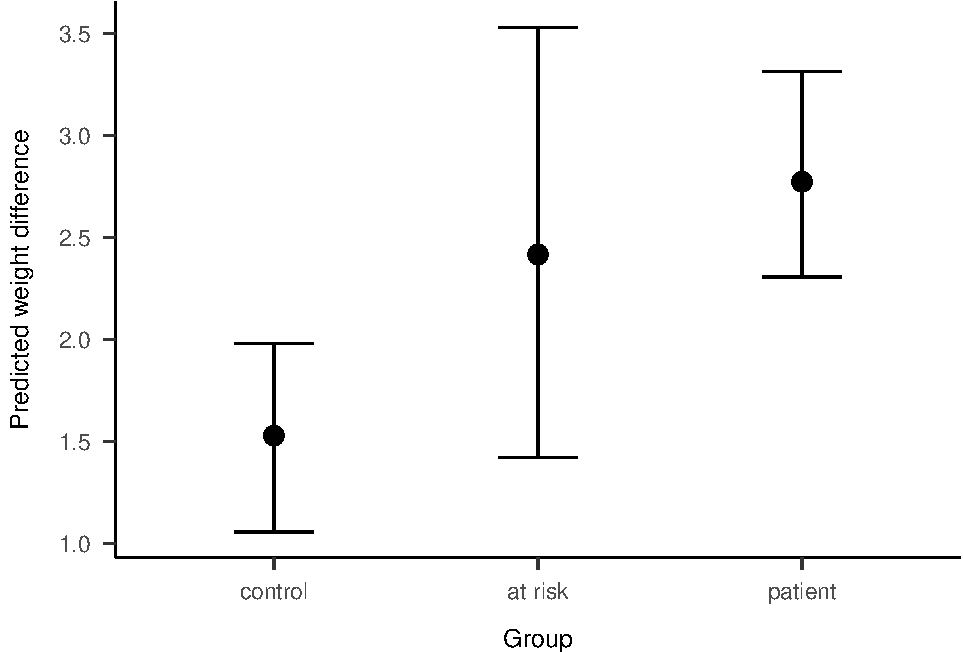
\includegraphics{046_weight_history_alpha_files/figure-latex/unnamed-chunk-16-1.pdf}

\begin{Shaded}
\begin{Highlighting}[]
\NormalTok{test\_right }\OtherTok{\textless{}{-}}\NormalTok{ bayestestR}\SpecialCharTok{::}\FunctionTok{bayesfactor\_parameters}\NormalTok{(m14, }\AttributeTok{direction =} \StringTok{"\textgreater{}"}\NormalTok{)}
\end{Highlighting}
\end{Shaded}

\begin{verbatim}
## Sampling priors, please wait...
\end{verbatim}

\begin{Shaded}
\begin{Highlighting}[]
\NormalTok{test\_right}
\end{Highlighting}
\end{Shaded}

\begin{verbatim}
## Bayes Factor (Savage-Dickey density ratio)
## 
## Parameter    |       BF
## -----------------------
## (Intercept)  | 1.05e+05
## Groupatrisk  |     1.94
## Grouppatient |   363.08
## 
## * Evidence Against The Null: 0
## *                 Direction: Right-Sided test
\end{verbatim}

Patients expect to gain more weight than controls; there is no evidence
of a difference between at-risk participants and controls. Summary
statistics

\begin{Shaded}
\begin{Highlighting}[]
\NormalTok{foo }\SpecialCharTok{\%\textgreater{}\%} 
  \FunctionTok{group\_by}\NormalTok{(Group) }\SpecialCharTok{\%\textgreater{}\%} 
  \FunctionTok{summarise}\NormalTok{(}
    \AttributeTok{avg\_rws =} \FunctionTok{mean}\NormalTok{(rws, }\AttributeTok{na.rm =} \ConstantTok{TRUE}\NormalTok{),}
    \AttributeTok{avg\_ws =} \FunctionTok{mean}\NormalTok{(ws, }\AttributeTok{na.rm =} \ConstantTok{TRUE}\NormalTok{),}
    \AttributeTok{n =} \FunctionTok{n}\NormalTok{()}
\NormalTok{  )}
\end{Highlighting}
\end{Shaded}

\begin{verbatim}
## # A tibble: 3 x 4
##   Group   avg_rws avg_ws     n
##   <fct>     <dbl>  <dbl> <int>
## 1 at risk  0.0767   5.75    12
## 2 control  0.0545   3.62    68
## 3 patient  0.130    7.48    37
\end{verbatim}

\end{document}
